\section{Binomial distributed values}
In the following subsections the performance of the different algorithms is tested for different kinds of inputs.
The exact distributions of the input are explained separately in each subsection.
The procedure for each comparison is always the same. A random input is generated according to the distribution and then solved by every algorithm.
All algorithms had the same two stopping conditions.
The first was reaching a perfect partition and the second was taking more than $100 \cdot n\ln(n)$ steps or $10 \cdot n\ln(n)$ in some cases.
For the lower values of $n$ the step limit of 100,000 was used instead.
For $n=200$ giving the algorithm only 600 steps is rather small.
In some cases the smaller inputs are even more difficult to solve.
Most modern computer should be able to handle 100,000 iterations in a short amount of time anyway.
So the minimum step limit of 100,000 seemed reasonable.
If either of these condition was met, the algorithm returned the current best solution.
This step is repeated 1000 times.
The results are presented in a table containing multiple statistics for each algorithm over all 1000 runs.
The data is explained in the table below.

\begin{tabular}{c|l}
      column name     & meaning                                                         \\ \hline
      algo type       & type of algorithm (RLS, RLS-N, RLS-R, (1+1)EA or pmut)          \\
      algo param      & parameter of the algorithm or '-' if it is the standard variant \\
      avg mut/change  & average \#bits flipped for iterations leading to an improvement \\
      avg mut/step    & average \#bits flipped for any iteration                        \\ \hline
      total avg count & average \#iterations for all runs                               \\
      avg eval count  & average \#iterations of runs returning an optimal solution      \\
      max eval count  & maximum \#iterations of runs returning an optimal solution      \\
      min eval count  & minimum \#iterations of runs returning an optimal solution      \\ \hline
      fails           & number of runs that did not find an optimal solution            \\
      fail ratio      & ratio of unsuccessful runs to all runs                          \\
      avg fail dif    & average value of $b_F-f(opt)$ for non-optimal solutions         \\
\end{tabular}

Firstly the different variants of the RLS are compared with values of $k \in\{2,3,4\}$, then the performance of the (1+1) EA with static mutation rate $c/n$ with $c \in\{1,2,3,5,10,50,100\}$ and lastly the performance of the $pmut_\beta$ mutation operator with the parameter $\beta \in \{-1.25, -1.5, \dots, -2.75,-3.0,-3.25\}$.
Additionally the best variants of each algorithm are compared in another 1000 runs.
Afterwards there is also a comparison for multiple input sizes of the best algorithms because the best algorithm is often dependent on the size of the input.
Normally there are three tables for each input.
The first states how often the algorithms did not find an optimal solution for the different input sizes ('fails' in top left cell).
The second gives their average performance for the successful runs ('avg' in top left cell) and the last the performance for all runs ('total avg' in top left cell).
The last two tables differ in the unsuccessful runs. Often the algorithm is stuck in a local optima it won't leave in reasonable time or never for variants of the RLS.
In these cases the step limit is the deciding factor on how big the penality for this run is.
So neither of the two average values alone is enough to give a complete insight on the performance.
Sometimes a variant of the RLS is much faster than the other algorithms for a specific input but is also the only algorithm to get stuck in a local optimum.
This creates the possibility to start the RLS variant with a low step limit and switch to the (1+1) EA if the RLS variant does not return an optimal solution.
Giving both tables for the different average values might help with this decision.

The first analysed inputs are inputs following a binomial distribution \textasciitilde$B(m,p)$ as those inputs have been researched in the previous subsection.
The results showed that the expected value of a single number is the main driver for the amount of perfect partitions the input has.
The results also suggested the inputs tend to have more perfect partitions if the expected value is lower.
The more perfect partitions an input has relative to the number of all possible partitions, the more likely the different RSHs are to find one of those.
Therefore researching inputs with higher expected values seems more interesting but generating higher values takes more time with a random number generator that needs $\mathcal{O}(mp)$ time.
To keep the time for generating one set of numbers reasonable the values chosen for all tests are $m=10000, p=0.1, n=10000$ with the expected value for a single number being $mp=1000$.
Figure~\ref{fig:binDistExample} shows a random binomial distributed input of length $n=10000$.
All elements are sharply concentrated around the expected value with all values being at $1000\pm200$.
So after reaching a difference between the two bins of below $(1000-200)/2=400$ the algorithm can no longer achieve an improvement by flipping a single bit.

\begin{figure}[h]
      \caption{Distribution of a random binomial input}
      \centering
      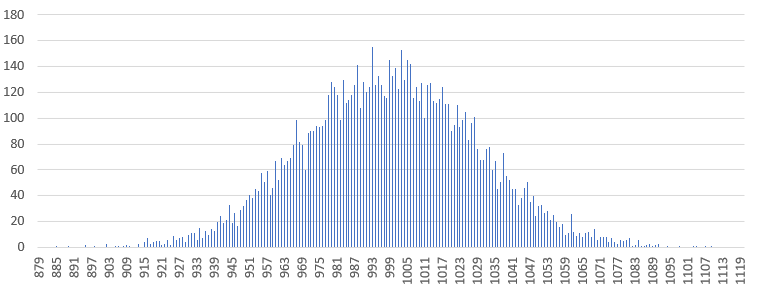
\includegraphics[width=0.7\textwidth]{figures/images/numberGenerator/binomialDistributionForN10000p0_1.png}\label{fig:binDistExample}
\end{figure}
\subsection{RLS Comparison}


\makebox[\linewidth]{
\begin{tabular}{lp{3cm}p{6cm}p{6cm}}
\begin{tabular}[h]{cccccccc}
algo type&            \RLSN&     \RLSR&     \RLSR&     \RLSN&     \RLSR&     \RLSN&       RLS\\
algo param&             b=2&       s=3&       s=4&       b=3&       s=2&       b=4&         -\\
avg mut/change&       2.000&     1.996&     2.476&     3.000&     1.502&     4.000&     1.000\\
avg mut/step&         2.000&     2.000&     2.500&     3.000&     1.500&     4.000&     1.000\\
\hline
total avg count&     83,118&   104,748&   105,513&   112,223&   114,486&   121,927& 2,443,567\\
avg eval count&      83,118&   104,748&   105,513&   112,223&   114,486&   121,927&    45,834\\
max eval count&     778,110& 1,453,252&   898,974& 1,377,471&   915,268&   816,633&   485,275\\
min eval count&         197&       126&        45&       212&       271&       155&       128\\
\hline
fail ratio&           0.000&     0.000&     0.000&     0.000&     0.000&     0.000&     0.447\\
avg fail dif&             -&         -&         -&         -&         -&         -&         1\\
\end{tabular}
\end{tabular}
}


The $\text{RLS-N}_2$ seems to perform the best as it mostly switches two elements which works great for binomial distributed inputs. 
The same algorithm with $k=4$ performs a bit worse but still good as switching 4 elements can be beneficial as well.
The variant of RLS-N with $k=3$ on the other hand does not reach the optimal solution in 23.4\% of the inputs with an average difference of 1.
It also needs 1000 times more iterations to find the optimal on average compared to the best algorithm $\text{RLS-N}_2$.
The RLS-R variants behave mostly the same with $k=2$ being the best, followed by $k=4$ and $k=3$.
In this case the variant of $k=3$ is by far not as bad as for the RLS-N because the probability of flipping 2 bits is 1/3 as compared to $\mathcal{O}(n^{-1})$ for the RLS-N.
The RLS-R seem all to be good option for binomial inputs with values of $k\in\{2,3,4\}$.
The RLS on the other hand performs by far the worst as it only moves one element at a time.
It only managed to reach the optimal solution once for 1000 different inputs.
The number of iterations for this input was only 50 so the RLS likely had a good initialisation with a few lucky steps leading directly to the optimum.
For all other cases the average difference between the bins was 254 which is close to the median of the values from 0 to $(1000-100)/2=450$.
This is likely due to the RLS being unable to improve the solution once the current solution has a difference below half of the lowest value.
\subsection{(1+1) EA Comparison}
For the (1+1) EA the best static mutation rate seems to be $3/n$. 
The probability of flipping 2 or 4 bits as n goes to infinity for mutation rate $1/n$ approaches $13/24e\approx 0.199$, for $2/n$ approaches $8/3e^2\approx 0.361$, for $3/n$ approaches $63/8e^3\approx 0.392$, for $4/n$ approaches $56/3e^4\approx 0.342$ and for $5/n$ approaches $77/2e^5\approx 0.259$. So the highest probability has $c=3$, followed by $c=4$ and $c=2$ then $c=5$ and lastly $c=1$. For higher values of $c$ the probability decreases further as the expected number of flipped bits is $c$ for mutation rate $c/n$.

\makebox[\linewidth]{
\begin{tabular}{lp{3cm}p{6cm}p{6cm}}
\begin{tabular}[h]{ccccccccc}
algo type&          (1+1) EA&   (1+1) EA&   (1+1) EA&   (1+1) EA&      (1+1) EA&   (1+1) EA&   (1+1) EA&   (1+1) EA\\
algo param&           3/n&     4/n&     2/n&     5/n&       -&    10/n&    50/n&   100/n\\
avg mut/change&     3.101&   3.968&   2.343&   4.859&   1.698&   9.732&  49.544&  99.494\\
avg mut/step&       2.999&   4.003&   2.002&   4.999&   1.001&   9.998&  49.998&  99.997\\
\hline
total avg count&      646&     701&     706&     857&   1,123&   1,508&   8,175&  15,485\\
avg eval count&       646&     701&     706&     857&   1,123&   1,508&   8,175&  15,485\\
max eval count&     5,346&   5,692&   3,415&   5,572&   7,001&  12,112&  52,831& 145,269\\
min eval count&        23&       4&      30&       9&      23&      14&      27&      69\\
\hline
fails&                  0&       0&       0&       0&       0&       0&       0&       0\\
fail ratio&         0.000&   0.000&   0.000&   0.000&   0.000&   0.000&   0.000&   0.000\\
avg fail dif&           -&       -&       -&       -&       -&       -&       -&       -\\
\end{tabular}
\end{tabular}
}


The static mutation rate $3/n$ seems to perform the best with both $4/n$ and $2/n$ being a close second place. The next best values are $5/n$ and the standard $1/n$ both having a clear difference between each other and the better parameters. From then on the number of iterations rises monotonically with rising mutation rate. The higher mutation rates perform significantly worse but the still find a solution within the limit as opposed to the standard RLS.
\subsection{pmut Comparison}


\makebox[\linewidth]{
\scriptsize
\begin{tabular}{lp{3cm}p{6cm}p{6cm}}
\begin{tabular}[h]{m{2.5cm}m{0,40cm}m{0,40cm}m{0,40cm}m{0,40cm}m{0,40cm}m{0,40cm}m{0,40cm}m{0,40cm}m{0,40cm}m{0,40cm}m{0,40cm}m{0,40cm}m{0,40cm}m{0,40cm}m{0,40cm}m{0,40cm}m{0,40cm}m{0,40cm}}
\multicolumn{1}{c}{algo type}&\multicolumn{2}{c}{            pmut}&\multicolumn{2}{c}{     pmut}&\multicolumn{2}{c}{     pmut}&\multicolumn{2}{c}{     pmut}&\multicolumn{2}{c}{     pmut}&\multicolumn{2}{c}{     pmut}&\multicolumn{2}{c}{     pmut}&\multicolumn{2}{c}{     pmut}&\multicolumn{2}{c}{     pmut}\\
\multicolumn{1}{c}{algo param}&\multicolumn{2}{c}{           3.25}&\multicolumn{2}{c}{     3.00}&\multicolumn{2}{c}{     2.75}&\multicolumn{2}{c}{     2.50}&\multicolumn{2}{c}{     2.25}&\multicolumn{2}{c}{     2.00}&\multicolumn{2}{c}{     1.75}&\multicolumn{2}{c}{     1.50}&\multicolumn{2}{c}{     1.25}\\
\multicolumn{1}{c}{avg mut/change}&\multicolumn{2}{c}{      1.583}&\multicolumn{2}{c}{    1.737}&\multicolumn{2}{c}{    2.002}&\multicolumn{2}{c}{    2.423}&\multicolumn{2}{c}{    3.303}&\multicolumn{2}{c}{    5.830}&\multicolumn{2}{c}{   12.519}&\multicolumn{2}{c}{   30.910}&\multicolumn{2}{c}{   73.182}\\
\multicolumn{1}{c}{avg mut/step}&\multicolumn{2}{c}{        1.729}&\multicolumn{2}{c}{    1.934}&\multicolumn{2}{c}{    2.274}&\multicolumn{2}{c}{    2.895}&\multicolumn{2}{c}{    4.360}&\multicolumn{2}{c}{    8.452}&\multicolumn{2}{c}{   22.278}&\multicolumn{2}{c}{   70.532}&\multicolumn{2}{c}{  224.421}\\
\hline
\multicolumn{1}{c}{avg eval count}&\multicolumn{2}{c}{        540}&\multicolumn{2}{c}{      569}&\multicolumn{2}{c}{      594}&\multicolumn{2}{c}{      641}&\multicolumn{2}{c}{      712}&\multicolumn{2}{c}{      808}&\multicolumn{2}{c}{      967}&\multicolumn{2}{c}{    1,285}&\multicolumn{2}{c}{    2,081}\\
\multicolumn{1}{c}{max eval count}&\multicolumn{2}{c}{      3,110}&\multicolumn{2}{c}{    2,891}&\multicolumn{2}{c}{    3,504}&\multicolumn{2}{c}{    3,896}&\multicolumn{2}{c}{    5,152}&\multicolumn{2}{c}{    4,274}&\multicolumn{2}{c}{    5,610}&\multicolumn{2}{c}{    6,190}&\multicolumn{2}{c}{   14,984}\\
\multicolumn{1}{c}{min eval count}&\multicolumn{2}{c}{         22}&\multicolumn{2}{c}{        9}&\multicolumn{2}{c}{       36}&\multicolumn{2}{c}{       25}&\multicolumn{2}{c}{       28}&\multicolumn{2}{c}{       27}&\multicolumn{2}{c}{       27}&\multicolumn{2}{c}{       13}&\multicolumn{2}{c}{       33}\\
\hline
\multicolumn{1}{c}{fail ratio}&\multicolumn{2}{c}{          0.000}&\multicolumn{2}{c}{    0.000}&\multicolumn{2}{c}{    0.000}&\multicolumn{2}{c}{    0.000}&\multicolumn{2}{c}{    0.000}&\multicolumn{2}{c}{    0.000}&\multicolumn{2}{c}{    0.000}&\multicolumn{2}{c}{    0.000}&\multicolumn{2}{c}{    0.000}\\
\hline
\multicolumn{1}{c}{p-value}&&\multicolumn{2}{c}{0.0000}&\multicolumn{2}{c}{0.0000}&\multicolumn{2}{c}{0.0000}&\multicolumn{2}{c}{0.0000}&\multicolumn{2}{c}{0.0000}&\multicolumn{2}{c}{0.0000}&\multicolumn{2}{c}{0.0000}&\multicolumn{2}{c}{0.0000}\\
&&&&&&&&&&&&&&&&&&\end{tabular}
\end{tabular}
}


For the $pmut_\beta$ mutation operator the choice of $\beta$ seems to be much more insignificant than for the RLS or (1+1) EA. Here all values perform comparably good with only the value of $\beta = -1.25$ having a clear performance difference compared to next best value. All values of $\beta$ reach an optimal solution in every case. The worst variant of the $pmut_\beta$ operator still performs much better than the worst value for the (1+1) EA and even better than the worst RLS variant. There is no clear winner but because $\beta=-2.25$ had the best performance in this experiment, it was used for the comparison of the best variants.
\subsection{Comparison of the best variants}


\makebox[\linewidth]{
\begin{tabular}{lp{3cm}p{6cm}p{6cm}}
\begin{tabular}[h]{cccc}
algo type&            RLS&    pmut&      EA\\
algo param&             -&    3.25&       -\\
avg mut/change&     1.000&   1.287&   1.272\\
avg mut/step&       1.000&   1.729&   1.000\\
\hline
avg eval count&    91,171& 143,121& 231,082\\
max eval count&   153,143& 227,737& 446,942\\
min eval count&    65,783&  93,602& 165,818\\
\hline
fail ratio&         0.000&   0.000&   0.000\\
\end{tabular}
\end{tabular}
}


For this setting of $m=10000, p=0.1, n=10000$ the RLS-N with $k=2$ performs better than the  (1+1) EA and $pmut_\beta$ mutation for all values of $c/n$ and $\beta$ by a factor of at least 2.
This is likely from the fact that this version of the RLS flips almost only two bits which seems to be close to optimal for this kind of input.
There are many values close to the expected value which can be switched to make small adjustments to the fitness value.
The (1+1) EA with $p=3/n$ and $pmut_\beta$ algorithm with $\beta=-2.25$ perform almost the same.
The (1+1) EA has a slightly lower average value but also has a higher minimum value and a higher maximum value.
To further investigate which input performs best on all binomial distributed inputs now a comparison with different input lengths follows.
The parameters of the distribution were not changed.\newline
The following table is the amount of runs in which the algorithms did not find an optimal solution within 50,000 steps.
The time limit was set 50,000 because the algorithm normally reach the optimal solution within a few thousand steps.
If the solutions is not found after 50,000 steps, the algorithm is most likely stuck in a local optimum which could only be left by flipping more bits than possible for the algorithm.

\begin{tabular}[h]{ccccccccc}
fails in 1000 runs&20&50&100&500&1000&5000&10000&50000\\\hline
RLS&984&773&411&1&0&0&0&0\\
\RLSR[2]&890&241&14&0&0&0&0&0\\
(1+1) EA (1$/n$)&711&75&5&0&0&0&0&0\\
(1+1) EA (2$/n$)&541&14&0&0&0&0&0&0\\
pmut (3.0)&566&63&4&0&0&0&0&0\\
pmut (3.25)&587&63&7&0&0&0&0&0\\
\end{tabular}


The (1+1) EA and $pmut_\beta$ always reach an optimal solution but the RLS does not.
The RLS variants that can only flip two steps per step perform significantly worse for small inputs.
They are probably more likely to get stuck in a local optimum where a step flipping 4 bits or more would be necessary.
So the RLS-N(2) does perform better for larger inputs but is much more likely to get stuck in a local optima.
The next table contains the average number of iterations the algorithm needed to find an optimal solution for all runs where the algorithms managed to find an optimal solution.
Here it still looks like the RLS-N(2) finds the solution with the lowest amount of steps, because the cases where the algorithm is stuck in a local optima are not contained in this table.

\begin{tabular}[h]{ccccccccc}
avg&20&50&100&500&1000&5000&10000&50000\\\hline
RLS&32&79&153&579&950&1859&1922&1797\\
\RLSR[2]&391&2124&5005&4218&3530&2362&2160&2229\\
(1+1) EA (1$/n$)&22471&18343&12834&8342&6511&3815&3458&3371\\
(1+1) EA (2$/n$)&16360&9243&6452&4503&4020&3171&3141&3133\\
pmut (3.25)&23440&15929&9658&5644&4406&2434&2162&2172\\
pmut (3.0)&21901&14696&9186&5222&4150&2510&2208&2213\\
\end{tabular}


The next table contains the overall average amount of iterations for every run.
So runs where no optimal was found add 50000 thousand to the sum of all iterations.

\begin{tabular}[h]{ccccccccc}
total avg&20&50&100&500&1000&5000&10000&50000\\\hline
RLS&99470&93459&74385&3474&447&389&421&555\\
\RLSR[2]&96305&63088&19364&815&589&565&595&699\\
(1+1) EA (1$/n$)&89444&52886&21141&1410&869&850&875&1046\\
(1+1) EA (2$/n$)&79603&37214&14107&1302&992&942&957&1055\\
pmut (3.25)&84226&48403&18280&930&542&526&546&642\\
pmut (3.0)&82474&46286&17825&917&576&548&573&668\\
\end{tabular}



Here the RLS-N(2) is only the best algorithm for values of $n \ge 500$.
Below this bound choosing the (1+1) EA with static mutation rate $3/n$ is a safer choice as the (1+1) EA reaches an optimal solution for every input (in this experiment).
\section{Geometric distributed values}
For the geometric distribution the chosen default value is $p=0.001$.
This results in an expected value of 1000 which is the same as for the binomial distribution in the last subsection.
This should make the results more comparable.
Another parameter is the maximum value which was set to $10 \cdot E(X)=10000$.
Theoretically with very low probability the geometric distribution could result in an almost endless loop with bad luck.
To prevent this issue the maximum value was inserted as an upper bound for the random number generator. 
Figure~\ref{fig:geoDistExample} shows that this maximum value does not change the input drastically as no value over 9000 was generated anyway.
The span of all values is way higher than for the binomial distribution, although they have same expected value.
Here the values are not in the interval $[800,1200]$ but rather between 0 and the maximum value. 

\begin{figure}[h]
      \caption{Distribution of a random geometric input}
      \centering
      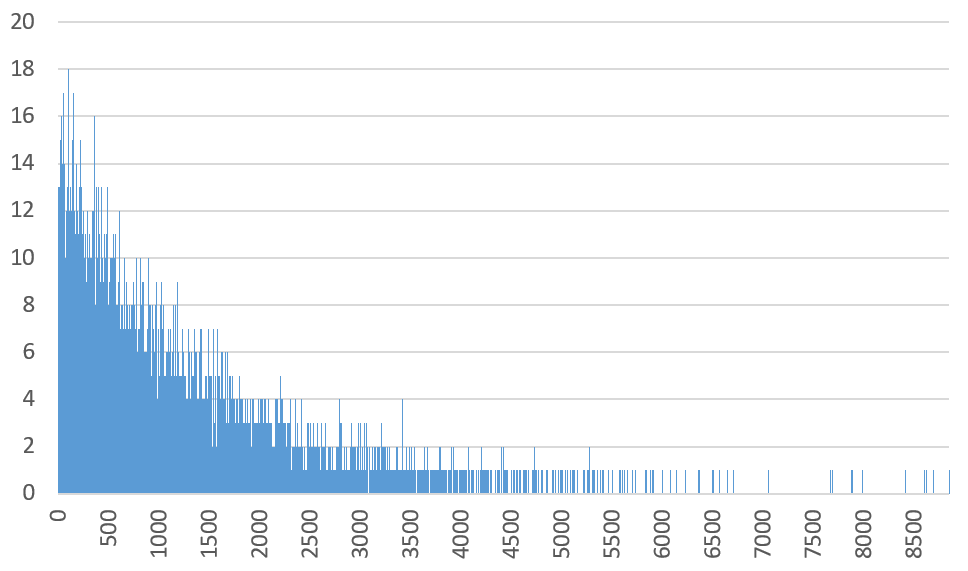
\includegraphics[width=0.7\textwidth]{figures/images/numberGenerator/geometricDistributionForp0_001.png}\label{fig:geoDistExample}
\end{figure}

The geometric distribution does not only have low values close or equal to 1 but also has mostly values that are very small.
This should lead to 1-bit flips being effective as the small values can remove the small differences. Because there are so many small values moving only one bit might be better than switching two elements.  
\subsection{RLS Comparison}


\makebox[\linewidth]{
\begin{tabular}{lp{3cm}p{6cm}p{6cm}}
\begin{tabular}[h]{cccccccc}
algo type&            \RLSN&     \RLSR&     \RLSR&     \RLSN&     \RLSR&     \RLSN&       RLS\\
algo param&             b=2&       s=3&       s=4&       b=3&       s=2&       b=4&         -\\
avg mut/change&       2.000&     1.996&     2.476&     3.000&     1.502&     4.000&     1.000\\
avg mut/step&         2.000&     2.000&     2.500&     3.000&     1.500&     4.000&     1.000\\
\hline
total avg count&     83,118&   104,748&   105,513&   112,223&   114,486&   121,927& 2,443,567\\
avg eval count&      83,118&   104,748&   105,513&   112,223&   114,486&   121,927&    45,834\\
max eval count&     778,110& 1,453,252&   898,974& 1,377,471&   915,268&   816,633&   485,275\\
min eval count&         197&       126&        45&       212&       271&       155&       128\\
\hline
fail ratio&           0.000&     0.000&     0.000&     0.000&     0.000&     0.000&     0.447\\
avg fail dif&             -&         -&         -&         -&         -&         -&         1\\
\end{tabular}
\end{tabular}
}


For these inputs the variants of the RLS perform differently to the binomial input.
The only similarity is the RLS being the worst as the RLS is the only algorithm that did not find an optimal solution for every input.
If the RLS did find an optimal solution in those 5 cases it would instead be the best RLS variant.
The other algorithms are ranked by the probability of flipping only one bit.
This means at first the three RLS-R variants from 2 to 3 to 4 and then the same for the RLS-N variants.
So it does seem like moving mostly one element at once is better for the geometric input in comparison to two elements for the binomial distribution.
In the 5 cases where the RLS did not find an optimal solution it was most likely stuck in a local optimum.

\subsection{(1+1) EA Comparison}


\makebox[\linewidth]{
\begin{tabular}{lp{3cm}p{6cm}p{6cm}}
\begin{tabular}[h]{ccccccccc}
algo type&          (1+1) EA&   (1+1) EA&   (1+1) EA&   (1+1) EA&      (1+1) EA&   (1+1) EA&   (1+1) EA&   (1+1) EA\\
algo param&           3/n&     4/n&     2/n&     5/n&       -&    10/n&    50/n&   100/n\\
avg mut/change&     3.101&   3.968&   2.343&   4.859&   1.698&   9.732&  49.544&  99.494\\
avg mut/step&       2.999&   4.003&   2.002&   4.999&   1.001&   9.998&  49.998&  99.997\\
\hline
total avg count&      646&     701&     706&     857&   1,123&   1,508&   8,175&  15,485\\
avg eval count&       646&     701&     706&     857&   1,123&   1,508&   8,175&  15,485\\
max eval count&     5,346&   5,692&   3,415&   5,572&   7,001&  12,112&  52,831& 145,269\\
min eval count&        23&       4&      30&       9&      23&      14&      27&      69\\
\hline
fails&                  0&       0&       0&       0&       0&       0&       0&       0\\
fail ratio&         0.000&   0.000&   0.000&   0.000&   0.000&   0.000&   0.000&   0.000\\
avg fail dif&           -&       -&       -&       -&       -&       -&       -&       -\\
\end{tabular}
\end{tabular}
}


The results for the (1+1) EA are similar to the results of the RLS. From mutation rate $3/n$ on the performance decreases with rising mutation rate.
The only part that does not fit into the theory of 1 bit flips being superior is the mutation rate $2/n$ performing better than the standard $1/n$.
The average number of iterations for the standard (1+1) EA is only slightly higher than for the mutation rate $2/n$, so this might be just due to a too small number of runs of the algorithms.
All variants reach an optimal solution within the given limit for the number of iterations.
\subsection{pmut Comparison}


\makebox[\linewidth]{
\scriptsize
\begin{tabular}{lp{3cm}p{6cm}p{6cm}}
\begin{tabular}[h]{m{2.5cm}m{0,40cm}m{0,40cm}m{0,40cm}m{0,40cm}m{0,40cm}m{0,40cm}m{0,40cm}m{0,40cm}m{0,40cm}m{0,40cm}m{0,40cm}m{0,40cm}m{0,40cm}m{0,40cm}m{0,40cm}m{0,40cm}m{0,40cm}m{0,40cm}}
\multicolumn{1}{c}{algo type}&\multicolumn{2}{c}{            pmut}&\multicolumn{2}{c}{     pmut}&\multicolumn{2}{c}{     pmut}&\multicolumn{2}{c}{     pmut}&\multicolumn{2}{c}{     pmut}&\multicolumn{2}{c}{     pmut}&\multicolumn{2}{c}{     pmut}&\multicolumn{2}{c}{     pmut}&\multicolumn{2}{c}{     pmut}\\
\multicolumn{1}{c}{algo param}&\multicolumn{2}{c}{           3.25}&\multicolumn{2}{c}{     3.00}&\multicolumn{2}{c}{     2.75}&\multicolumn{2}{c}{     2.50}&\multicolumn{2}{c}{     2.25}&\multicolumn{2}{c}{     2.00}&\multicolumn{2}{c}{     1.75}&\multicolumn{2}{c}{     1.50}&\multicolumn{2}{c}{     1.25}\\
\multicolumn{1}{c}{avg mut/change}&\multicolumn{2}{c}{      1.583}&\multicolumn{2}{c}{    1.737}&\multicolumn{2}{c}{    2.002}&\multicolumn{2}{c}{    2.423}&\multicolumn{2}{c}{    3.303}&\multicolumn{2}{c}{    5.830}&\multicolumn{2}{c}{   12.519}&\multicolumn{2}{c}{   30.910}&\multicolumn{2}{c}{   73.182}\\
\multicolumn{1}{c}{avg mut/step}&\multicolumn{2}{c}{        1.729}&\multicolumn{2}{c}{    1.934}&\multicolumn{2}{c}{    2.274}&\multicolumn{2}{c}{    2.895}&\multicolumn{2}{c}{    4.360}&\multicolumn{2}{c}{    8.452}&\multicolumn{2}{c}{   22.278}&\multicolumn{2}{c}{   70.532}&\multicolumn{2}{c}{  224.421}\\
\hline
\multicolumn{1}{c}{avg eval count}&\multicolumn{2}{c}{        540}&\multicolumn{2}{c}{      569}&\multicolumn{2}{c}{      594}&\multicolumn{2}{c}{      641}&\multicolumn{2}{c}{      712}&\multicolumn{2}{c}{      808}&\multicolumn{2}{c}{      967}&\multicolumn{2}{c}{    1,285}&\multicolumn{2}{c}{    2,081}\\
\multicolumn{1}{c}{max eval count}&\multicolumn{2}{c}{      3,110}&\multicolumn{2}{c}{    2,891}&\multicolumn{2}{c}{    3,504}&\multicolumn{2}{c}{    3,896}&\multicolumn{2}{c}{    5,152}&\multicolumn{2}{c}{    4,274}&\multicolumn{2}{c}{    5,610}&\multicolumn{2}{c}{    6,190}&\multicolumn{2}{c}{   14,984}\\
\multicolumn{1}{c}{min eval count}&\multicolumn{2}{c}{         22}&\multicolumn{2}{c}{        9}&\multicolumn{2}{c}{       36}&\multicolumn{2}{c}{       25}&\multicolumn{2}{c}{       28}&\multicolumn{2}{c}{       27}&\multicolumn{2}{c}{       27}&\multicolumn{2}{c}{       13}&\multicolumn{2}{c}{       33}\\
\hline
\multicolumn{1}{c}{fail ratio}&\multicolumn{2}{c}{          0.000}&\multicolumn{2}{c}{    0.000}&\multicolumn{2}{c}{    0.000}&\multicolumn{2}{c}{    0.000}&\multicolumn{2}{c}{    0.000}&\multicolumn{2}{c}{    0.000}&\multicolumn{2}{c}{    0.000}&\multicolumn{2}{c}{    0.000}&\multicolumn{2}{c}{    0.000}\\
\hline
\multicolumn{1}{c}{p-value}&&\multicolumn{2}{c}{0.0000}&\multicolumn{2}{c}{0.0000}&\multicolumn{2}{c}{0.0000}&\multicolumn{2}{c}{0.0000}&\multicolumn{2}{c}{0.0000}&\multicolumn{2}{c}{0.0000}&\multicolumn{2}{c}{0.0000}&\multicolumn{2}{c}{0.0000}\\
&&&&&&&&&&&&&&&&&&\end{tabular}
\end{tabular}
}


The results for the $pmut_\beta$ operator are even more clear than for the (1+1) EA.
With increasing values (decreasing absolute values) for $\beta$ the amounts of flipped bits per step increases.
The performance on the other hand decreases with rising values for $\beta$ which fits into the theory of one bit flips being better for gemoetric distributed inputs.
The only special case that does not support this theory is the value $\beta=-2.5$ performing better than $\beta=-2.75$.
Here the same might hold as for the (1+1) EA.
The number of repetitions of the algorithm might simply be too small to make the small difference in the performance between the two values visible.
The difference in the performance for the $pmut_\beta$ operator is not as drastic as for the (1+1) EA.
Only $\beta=-1.25$ performs significantly worse the next best value.

\subsection{Comparison of the best variants}


\makebox[\linewidth]{
\begin{tabular}{lp{3cm}p{6cm}p{6cm}}
\begin{tabular}[h]{cccc}
algo type&            RLS&    pmut&      EA\\
algo param&             -&    3.25&       -\\
avg mut/change&     1.000&   1.287&   1.272\\
avg mut/step&       1.000&   1.729&   1.000\\
\hline
avg eval count&    91,171& 143,121& 231,082\\
max eval count&   153,143& 227,737& 446,942\\
min eval count&    65,783&  93,602& 165,818\\
\hline
fail ratio&         0.000&   0.000&   0.000\\
\end{tabular}
\end{tabular}
}


For the geometric distribution once again a variant of the RLS performs the best.
The $pmut_{-3.25}$ performs almost equally good with only the (1+1) EA variant performing clearly worse.
Here the algorithms are sorted again by their average number of flips per steps.
The theory of flipping one bit per step being better seems to be true for this kind of input.\newline
To further confirm the best choice for this kind of input there was another experiment of the best variants.
The setup is mostly the same except for having a fixed time limit of 100,000 instead of using $100 \cdot n\ln(n)$ as the limit.
The smaller inputs are harder relative to their input size so using $100 \cdot n\ln(n)$ as a bound is too small.
The first try was executed with 50,000 as the step limit but there the algorithms performed too bad for $n=20$.
Therefore for the second attempt the step limit was increased to 100,000.
The first table lists the number of runs where the different algorithms did not find the optimal solution within the time limit.

\begin{tabular}[h]{ccccccccc}
fails in 1000 runs&20&50&100&500&1000&5000&10000&50000\\\hline
RLS&984&773&411&1&0&0&0&0\\
\RLSR[2]&890&241&14&0&0&0&0&0\\
(1+1) EA (1$/n$)&711&75&5&0&0&0&0&0\\
(1+1) EA (2$/n$)&541&14&0&0&0&0&0&0\\
pmut (3.0)&566&63&4&0&0&0&0&0\\
pmut (3.25)&587&63&7&0&0&0&0&0\\
\end{tabular}


For small inputs the geometric distributed input seems to be likely to not have a perfect partition or only very few because there were many iterations where neither of the algorithms found an optimal solution within the time limit.
It seems many of the algorithms especially the variants of the RLS seem to be likely to get stuck in a local optima.
The (1+1) finds an optimum in most of the runs, so the geometric distributed inputs also seem to be likely to have a perfect partition for small values.
They are definitely not as solvable as the binomial inputs but they still have a perfect partition most times.
The next table visualises the average number of iterations the algorithms needed for finding an optimal solution if the algorithm managed to do so.

\begin{tabular}[h]{ccccccccc}
avg&20&50&100&500&1000&5000&10000&50000\\\hline
RLS&32&79&153&579&950&1859&1922&1797\\
\RLSR[2]&391&2124&5005&4218&3530&2362&2160&2229\\
(1+1) EA (1$/n$)&22471&18343&12834&8342&6511&3815&3458&3371\\
(1+1) EA (2$/n$)&16360&9243&6452&4503&4020&3171&3141&3133\\
pmut (3.25)&23440&15929&9658&5644&4406&2434&2162&2172\\
pmut (3.0)&21901&14696&9186&5222&4150&2510&2208&2213\\
\end{tabular}


The variants of the (1+1) EA and of the $pmut$ algorithm seem to take about 20,000 iterations for $n=20$ if they manage to find the optimal solution.
They also perform better and better the lager the input gets.
This is probability caused by the many additional small values that can be used for smaller adjustments to the fitness.
Also a really high value does not have as much of an input, because there are possibly other larger values which cancel each other out, if they are in different bins.
The last table again lists the total average number of steps.

\begin{tabular}[h]{ccccccccc}
total avg&20&50&100&500&1000&5000&10000&50000\\\hline
RLS&99470&93459&74385&3474&447&389&421&555\\
\RLSR[2]&96305&63088&19364&815&589&565&595&699\\
(1+1) EA (1$/n$)&89444&52886&21141&1410&869&850&875&1046\\
(1+1) EA (2$/n$)&79603&37214&14107&1302&992&942&957&1055\\
pmut (3.25)&84226&48403&18280&930&542&526&546&642\\
pmut (3.0)&82474&46286&17825&917&576&548&573&668\\
\end{tabular}



The RLS is only an option if the input is large enough $n \ge 10,000$. For smaller input sizes especially for $n \le 100$ choosing the (1+1) EA with mutation rate $2/n$ seems like the best choice. For larger values this (1+1) EA does not find an optimal solution the fastest but is still fast enough to be a viable option. Another rather save option is $pmut_{-3.25}$. This algorithm performs worse for $n \le 100$ but is still good in comparison to the other algorithms. For $n \ge 1000$ $pmut_{-3.25}$ starts to outperform the best version of the (1+1) EA and almost all other researched algorithms.
\section{Uniform distributed inputs}
For the uniform distribution the default values were 1 for the lower bound and 50000 for the upper bound (exclusive).
The range was limited to 50000 to reduce the time the algorithms needs to find an optimal solution.
The higher the values are with too few values the more likely the input is to not have a perfect partition\cite{borgs2001phase}.
This will cause the algorithms to always reach the limit for the number of iterations which drastically increases the time needed for the experiment.
The length of the input was 50000.


\begin{figure}[h]
      \caption{Distribution of a random uniform input (10000 values between 1 and 100)}
      \centering
      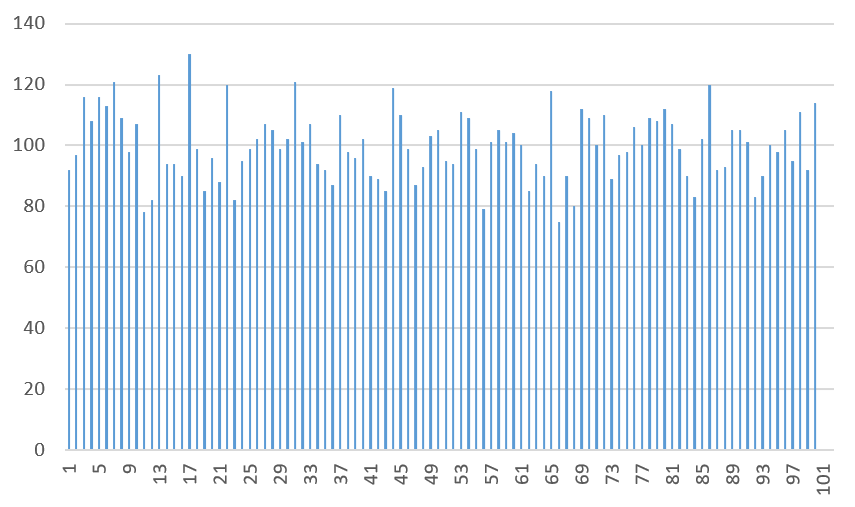
\includegraphics[width=0.7\textwidth]{figures/images/numberGenerator/uniformDistributionMin1Max101n10000.png}\label{fig:uniDistExample}
\end{figure}
\subsection{RLS Comparison}


\makebox[\linewidth]{
\begin{tabular}{lp{3cm}p{6cm}p{6cm}}
\begin{tabular}[h]{cccccccc}
algo type&            \RLSN&     \RLSR&     \RLSR&     \RLSN&     \RLSR&     \RLSN&       RLS\\
algo param&             b=2&       s=3&       s=4&       b=3&       s=2&       b=4&         -\\
avg mut/change&       2.000&     1.996&     2.476&     3.000&     1.502&     4.000&     1.000\\
avg mut/step&         2.000&     2.000&     2.500&     3.000&     1.500&     4.000&     1.000\\
\hline
total avg count&     83,118&   104,748&   105,513&   112,223&   114,486&   121,927& 2,443,567\\
avg eval count&      83,118&   104,748&   105,513&   112,223&   114,486&   121,927&    45,834\\
max eval count&     778,110& 1,453,252&   898,974& 1,377,471&   915,268&   816,633&   485,275\\
min eval count&         197&       126&        45&       212&       271&       155&       128\\
\hline
fail ratio&           0.000&     0.000&     0.000&     0.000&     0.000&     0.000&     0.447\\
avg fail dif&             -&         -&         -&         -&         -&         -&         1\\
\end{tabular}
\end{tabular}
}


The picture for the RLS variants on this type of input is not clear.
There in no obvious tendency for neither of the variants.
The only obvious thing is the RLS being the worst of the RLS variants again.
Every variant reaches the optimal solution in every case except for the RLS which only manages for 44.7 \% of the inputs.
The RLS-N(2) seems to be the best variant for these kinds of inputs.
The next best variants are the RLS-(R) with $k=3$ and $k=4$ which only differ by 1 \%.

\subsection{(1+1) EA Comparison}


\makebox[\linewidth]{
\begin{tabular}{lp{3cm}p{6cm}p{6cm}}
\begin{tabular}[h]{ccccccccc}
algo type&          (1+1) EA&   (1+1) EA&   (1+1) EA&   (1+1) EA&      (1+1) EA&   (1+1) EA&   (1+1) EA&   (1+1) EA\\
algo param&           3/n&     4/n&     2/n&     5/n&       -&    10/n&    50/n&   100/n\\
avg mut/change&     3.101&   3.968&   2.343&   4.859&   1.698&   9.732&  49.544&  99.494\\
avg mut/step&       2.999&   4.003&   2.002&   4.999&   1.001&   9.998&  49.998&  99.997\\
\hline
total avg count&      646&     701&     706&     857&   1,123&   1,508&   8,175&  15,485\\
avg eval count&       646&     701&     706&     857&   1,123&   1,508&   8,175&  15,485\\
max eval count&     5,346&   5,692&   3,415&   5,572&   7,001&  12,112&  52,831& 145,269\\
min eval count&        23&       4&      30&       9&      23&      14&      27&      69\\
\hline
fails&                  0&       0&       0&       0&       0&       0&       0&       0\\
fail ratio&         0.000&   0.000&   0.000&   0.000&   0.000&   0.000&   0.000&   0.000\\
avg fail dif&           -&       -&       -&       -&       -&       -&       -&       -\\
\end{tabular}
\end{tabular}
}


The (1+1) EA seems to perform better with a lower mutation rate.
The vales $p_m=2/n$ and $p_m=3/n$ reach an optimal solution equally fast.
From then on speed of convergence decreases with increasing mutation rate.
The only exception from this case is the (1+1) EA which performs the worst despite having the lowest mutation rate.
For the uniform distributed input all variants of the (1+1) EA reach an optimal solution within the step limit as for the previous input types.
\subsection{pmut Comparison}


\makebox[\linewidth]{
\scriptsize
\begin{tabular}{lp{3cm}p{6cm}p{6cm}}
\begin{tabular}[h]{m{2.5cm}m{0,40cm}m{0,40cm}m{0,40cm}m{0,40cm}m{0,40cm}m{0,40cm}m{0,40cm}m{0,40cm}m{0,40cm}m{0,40cm}m{0,40cm}m{0,40cm}m{0,40cm}m{0,40cm}m{0,40cm}m{0,40cm}m{0,40cm}m{0,40cm}}
\multicolumn{1}{c}{algo type}&\multicolumn{2}{c}{            pmut}&\multicolumn{2}{c}{     pmut}&\multicolumn{2}{c}{     pmut}&\multicolumn{2}{c}{     pmut}&\multicolumn{2}{c}{     pmut}&\multicolumn{2}{c}{     pmut}&\multicolumn{2}{c}{     pmut}&\multicolumn{2}{c}{     pmut}&\multicolumn{2}{c}{     pmut}\\
\multicolumn{1}{c}{algo param}&\multicolumn{2}{c}{           3.25}&\multicolumn{2}{c}{     3.00}&\multicolumn{2}{c}{     2.75}&\multicolumn{2}{c}{     2.50}&\multicolumn{2}{c}{     2.25}&\multicolumn{2}{c}{     2.00}&\multicolumn{2}{c}{     1.75}&\multicolumn{2}{c}{     1.50}&\multicolumn{2}{c}{     1.25}\\
\multicolumn{1}{c}{avg mut/change}&\multicolumn{2}{c}{      1.583}&\multicolumn{2}{c}{    1.737}&\multicolumn{2}{c}{    2.002}&\multicolumn{2}{c}{    2.423}&\multicolumn{2}{c}{    3.303}&\multicolumn{2}{c}{    5.830}&\multicolumn{2}{c}{   12.519}&\multicolumn{2}{c}{   30.910}&\multicolumn{2}{c}{   73.182}\\
\multicolumn{1}{c}{avg mut/step}&\multicolumn{2}{c}{        1.729}&\multicolumn{2}{c}{    1.934}&\multicolumn{2}{c}{    2.274}&\multicolumn{2}{c}{    2.895}&\multicolumn{2}{c}{    4.360}&\multicolumn{2}{c}{    8.452}&\multicolumn{2}{c}{   22.278}&\multicolumn{2}{c}{   70.532}&\multicolumn{2}{c}{  224.421}\\
\hline
\multicolumn{1}{c}{avg eval count}&\multicolumn{2}{c}{        540}&\multicolumn{2}{c}{      569}&\multicolumn{2}{c}{      594}&\multicolumn{2}{c}{      641}&\multicolumn{2}{c}{      712}&\multicolumn{2}{c}{      808}&\multicolumn{2}{c}{      967}&\multicolumn{2}{c}{    1,285}&\multicolumn{2}{c}{    2,081}\\
\multicolumn{1}{c}{max eval count}&\multicolumn{2}{c}{      3,110}&\multicolumn{2}{c}{    2,891}&\multicolumn{2}{c}{    3,504}&\multicolumn{2}{c}{    3,896}&\multicolumn{2}{c}{    5,152}&\multicolumn{2}{c}{    4,274}&\multicolumn{2}{c}{    5,610}&\multicolumn{2}{c}{    6,190}&\multicolumn{2}{c}{   14,984}\\
\multicolumn{1}{c}{min eval count}&\multicolumn{2}{c}{         22}&\multicolumn{2}{c}{        9}&\multicolumn{2}{c}{       36}&\multicolumn{2}{c}{       25}&\multicolumn{2}{c}{       28}&\multicolumn{2}{c}{       27}&\multicolumn{2}{c}{       27}&\multicolumn{2}{c}{       13}&\multicolumn{2}{c}{       33}\\
\hline
\multicolumn{1}{c}{fail ratio}&\multicolumn{2}{c}{          0.000}&\multicolumn{2}{c}{    0.000}&\multicolumn{2}{c}{    0.000}&\multicolumn{2}{c}{    0.000}&\multicolumn{2}{c}{    0.000}&\multicolumn{2}{c}{    0.000}&\multicolumn{2}{c}{    0.000}&\multicolumn{2}{c}{    0.000}&\multicolumn{2}{c}{    0.000}\\
\hline
\multicolumn{1}{c}{p-value}&&\multicolumn{2}{c}{0.0000}&\multicolumn{2}{c}{0.0000}&\multicolumn{2}{c}{0.0000}&\multicolumn{2}{c}{0.0000}&\multicolumn{2}{c}{0.0000}&\multicolumn{2}{c}{0.0000}&\multicolumn{2}{c}{0.0000}&\multicolumn{2}{c}{0.0000}\\
&&&&&&&&&&&&&&&&&&\end{tabular}
\end{tabular}
}


The optimal value for $\beta$ seems to be somewhere around -2.0 to -2.5.
The values next to this interval start to decrease in both directions, but -1.75 and -2.75 are still relatively close to the performance of the optimal value.
The values equally wide apart from -2.25 perform equally good.

\subsection{Comparison of the best variants}


\makebox[\linewidth]{
\begin{tabular}{lp{3cm}p{6cm}p{6cm}}
\begin{tabular}[h]{cccc}
algo type&            RLS&    pmut&      EA\\
algo param&             -&    3.25&       -\\
avg mut/change&     1.000&   1.287&   1.272\\
avg mut/step&       1.000&   1.729&   1.000\\
\hline
avg eval count&    91,171& 143,121& 231,082\\
max eval count&   153,143& 227,737& 446,942\\
min eval count&    65,783&  93,602& 165,818\\
\hline
fail ratio&         0.000&   0.000&   0.000\\
\end{tabular}
\end{tabular}
}


For the uniform distributed input the best variant of the RLS once again seems to have the best variant.
But by looking at the smaller values again this does not hold in general.

\begin{tabular}[h]{ccccccccc}
fails in 1000 runs&20&50&100&500&1000&5000&10000&50000\\\hline
RLS&984&773&411&1&0&0&0&0\\
\RLSR[2]&890&241&14&0&0&0&0&0\\
(1+1) EA (1$/n$)&711&75&5&0&0&0&0&0\\
(1+1) EA (2$/n$)&541&14&0&0&0&0&0&0\\
pmut (3.0)&566&63&4&0&0&0&0&0\\
pmut (3.25)&587&63&7&0&0&0&0&0\\
\end{tabular}


The RLS variants are the most likely to get stuck in a local optimum for $n\le100$. The (1+1) EA variants also often do not find an optimal solution, but this happens less frequently. The more values the input has the more likely it is for any of the algorithms to find a perfect partition. Between $n=100$ and $n=500$ the performance of the RLS-N(2) drastically increases and for $n\ge500$ this variant of the RLS stays the best variant for the remaining input sizes.

\begin{tabular}[h]{ccccccccc}
avg&20&50&100&500&1000&5000&10000&50000\\\hline
RLS&32&79&153&579&950&1859&1922&1797\\
\RLSR[2]&391&2124&5005&4218&3530&2362&2160&2229\\
(1+1) EA (1$/n$)&22471&18343&12834&8342&6511&3815&3458&3371\\
(1+1) EA (2$/n$)&16360&9243&6452&4503&4020&3171&3141&3133\\
pmut (3.25)&23440&15929&9658&5644&4406&2434&2162&2172\\
pmut (3.0)&21901&14696&9186&5222&4150&2510&2208&2213\\
\end{tabular}


The steps needed to find an optimal solution seems to be nearly constant for every algorithm as the number of steps does not strictly increase with $n$ but sometimes even decreases for $n\le1000$.
This is caused by the number of steps the algorithm was given.
For $n\le1000$ the step size was 100000 and for the bigger values it was $10n\ln(n)$.
Interestingly enough the average number of steps decreases from $n=10000$ to $n=50000$ for most algorithms.

\begin{tabular}[h]{ccccccccc}
total avg&20&50&100&500&1000&5000&10000&50000\\\hline
RLS&99470&93459&74385&3474&447&389&421&555\\
\RLSR[2]&96305&63088&19364&815&589&565&595&699\\
(1+1) EA (1$/n$)&89444&52886&21141&1410&869&850&875&1046\\
(1+1) EA (2$/n$)&79603&37214&14107&1302&992&942&957&1055\\
pmut (3.25)&84226&48403&18280&930&542&526&546&642\\
pmut (3.0)&82474&46286&17825&917&576&548&573&668\\
\end{tabular}



My general advice would be choosing the RLS-N(2) for $n\ge500$ and the (1+1) EA with $p_m=4/n$ otherwise.
\section{powerlaw distributed inputs}
This distribution has mostly small values, but occasionally it also generates bigger values.
The higher (absolute lower) the parameter the higher the values get and also the amount of big values increases.
For a parameter of $\beta=-2.75$ the distribution looks like in Figure~\ref{fig:powerDistExample1}.

\begin{figure}[h]
      \caption{Distribution of a random powerlaw input with $\beta=-2.75$}
      \centering
      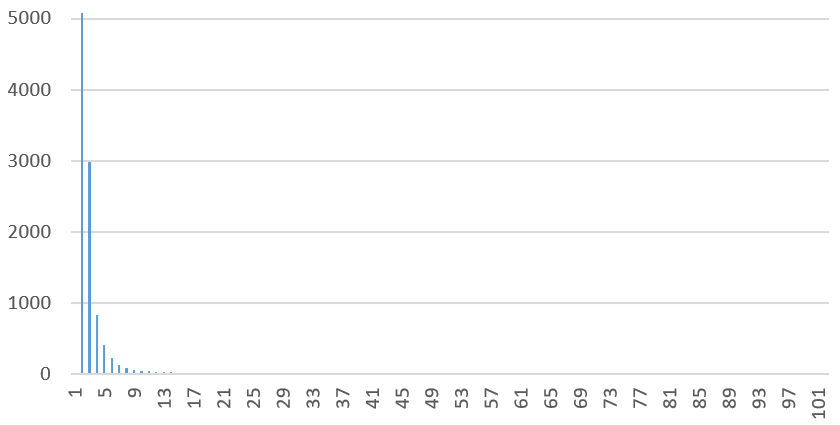
\includegraphics[width=0.7\textwidth]{figures/images/numberGenerator/powerlaw_-2_75.png}\label{fig:powerDistExample1}
\end{figure}

For a value of $\beta=-1.25$ the distribution looks a bit different.
There are less small values close to one and instead also big values even over 1000.
Figure~\ref{fig:powerDistExample2} is cropped to get a more clear view for the smaller values.
The higher values mostly occurred 0 to 2 times.
The highest value 8848 occurred only once.

\begin{figure}[h]
      \caption{Distribution of a random powerlaw input with $\beta=-1.25$}
      \centering
      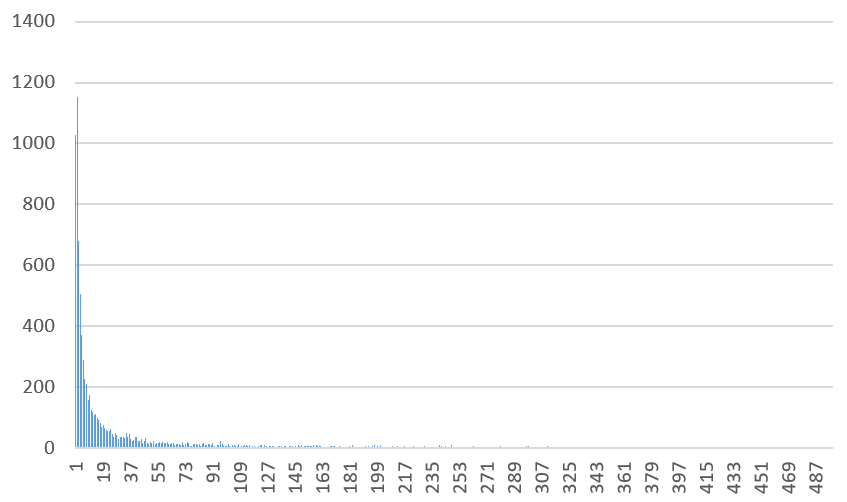
\includegraphics[width=0.7\textwidth]{figures/images/numberGenerator/powerlaw_-1_25.png}\label{fig:powerDistExample2}
\end{figure}
\subsection{RLS Comparison}
The following table lists the results for the RLS for inputs that are chosen from a powerlaw distribution with $\beta=-2.75$.


\makebox[\linewidth]{
\begin{tabular}{lp{3cm}p{6cm}p{6cm}}
\begin{tabular}[h]{cccccccc}
algo type&            \RLSN&     \RLSR&     \RLSR&     \RLSN&     \RLSR&     \RLSN&       RLS\\
algo param&             b=2&       s=3&       s=4&       b=3&       s=2&       b=4&         -\\
avg mut/change&       2.000&     1.996&     2.476&     3.000&     1.502&     4.000&     1.000\\
avg mut/step&         2.000&     2.000&     2.500&     3.000&     1.500&     4.000&     1.000\\
\hline
total avg count&     83,118&   104,748&   105,513&   112,223&   114,486&   121,927& 2,443,567\\
avg eval count&      83,118&   104,748&   105,513&   112,223&   114,486&   121,927&    45,834\\
max eval count&     778,110& 1,453,252&   898,974& 1,377,471&   915,268&   816,633&   485,275\\
min eval count&         197&       126&        45&       212&       271&       155&       128\\
\hline
fail ratio&           0.000&     0.000&     0.000&     0.000&     0.000&     0.000&     0.447\\
avg fail dif&             -&         -&         -&         -&         -&         -&         1\\
\end{tabular}
\end{tabular}
}


Due to the many small values and all values being relatively small in general the higher mutation rates perform better.
So the algorithms are ranked by the amount of bits they flip in an average step.
For this parameter the input is relatively easy as all variants manage to find an optimal solution in 400 steps on average for an input size of 20,000.
The next table lists the results for $\beta=-1.25$ and an input size of 10,000.

\makebox[\linewidth]{
\begin{tabular}{lp{3cm}p{6cm}p{6cm}}
\begin{tabular}[h]{cccccccc}
algo type&           RLS-R&    RLS-R&    RLS-N&    RLS-N&    RLS-R&    RLS-N&      RLS\\
algo param&            r=4&      r=3&      n=3&      n=2&      r=2&      n=4&        -\\
avg mut/change&      2.445&    1.967&    3.000&    2.000&    1.486&    4.000&    1.000\\
avg mut/step&        2.500&    2.001&    3.000&    2.000&    1.500&    4.000&    1.000\\
\hline
total avg count&       255&      272&      284&      286&      330&      370&      434\\
avg eval count&        255&      272&      284&      286&      330&      370&      434\\
max eval count&        847&      885&    1,553&    1,149&    1,130&    1,879&    1,911\\
min eval count&         26&       25&       36&       15&       12&       29&       26\\
\hline
fails&                   0&        0&        0&        0&        0&        0&        0\\
fail ratio&          0.000&    0.000&    0.000&    0.000&    0.000&    0.000&    0.000\\
avg fail dif&            -&        -&        -&        -&        -&        -&        -\\
\end{tabular}
\end{tabular}
}


The input is still easy to solve for the RLS variants, but the concept of the more bits flipped the better does not hold any more.
So the optimal parameter for a specific type of input is only fixed for the specific parameters of this distribution.
Generally the RLS-R variants seem to perform good for the different parameters of the distribution especially with increasing value of $k$.
\subsection{(1+1) EA Comparison}
The first table again shows the results for parameter $\beta=-2.75$

\makebox[\linewidth]{
\begin{tabular}{lp{3cm}p{6cm}p{6cm}}
\begin{tabular}[h]{ccccccccc}
algo type&          (1+1) EA&   (1+1) EA&   (1+1) EA&   (1+1) EA&      (1+1) EA&   (1+1) EA&   (1+1) EA&   (1+1) EA\\
algo param&           3/n&     4/n&     2/n&     5/n&       -&    10/n&    50/n&   100/n\\
avg mut/change&     3.101&   3.968&   2.343&   4.859&   1.698&   9.732&  49.544&  99.494\\
avg mut/step&       2.999&   4.003&   2.002&   4.999&   1.001&   9.998&  49.998&  99.997\\
\hline
total avg count&      646&     701&     706&     857&   1,123&   1,508&   8,175&  15,485\\
avg eval count&       646&     701&     706&     857&   1,123&   1,508&   8,175&  15,485\\
max eval count&     5,346&   5,692&   3,415&   5,572&   7,001&  12,112&  52,831& 145,269\\
min eval count&        23&       4&      30&       9&      23&      14&      27&      69\\
\hline
fails&                  0&       0&       0&       0&       0&       0&       0&       0\\
fail ratio&         0.000&   0.000&   0.000&   0.000&   0.000&   0.000&   0.000&   0.000\\
avg fail dif&           -&       -&       -&       -&       -&       -&       -&       -\\
\end{tabular}
\end{tabular}
}


Here the same rule holds for the RLS to some extent.
Until $p_m\le50/n$ the speed of convergence increases but at $p_m=100/n$ the speed decreases again.
The optimal value seems to be somewhere between around $p_m=50/n$.
The (1+1) variants are generally faster than all RLS variants when comparing the maximum number of iterations.
For mutation rates $3/n\le p_m \le 100/n$ the (1+1) EA is also faster on average.
The next table shows the results for a powerlaw distribution with $\beta=-1.25$.

\makebox[\linewidth]{
\begin{tabular}{lp{3cm}p{6cm}p{6cm}}
\begin{tabular}[h]{ccccccccc}
algo type&             EA-SM&      EA-SM&      EA-SM&      EA-SM&         EA&      EA-SM&      EA-SM&      EA-SM\\
algo param&              4/n&        3/n&        2/n&        5/n&          -&       10/n&       50/n&      100/n\\
avg mut/change&        3.913&      3.061&      2.255&      4.794&      1.559&      9.489&     49.461&     99.590\\
avg mut/step&          4.005&      2.999&      2.001&      4.999&      1.000&      9.997&     50.001&    100.000\\
\hline
total avg count&         243&        245&        291&        299&        509&      1,248&     53,071&     99,580\\
avg eval count&          243&        245&        291&        299&        509&      1,248&     53,071&     97,933\\
max eval count&        1,107&        752&        949&      1,258&      1,701&      9,332&    530,320&    753,937\\
min eval count&           23&          4&         15&         17&         50&         26&        213&        121\\
\hline
fails&                     0&          0&          0&          0&          0&          0&          0&          2\\
fail ratio&            0.000&      0.000&      0.000&      0.000&      0.000&      0.000&      0.000&      0.002\\
avg fail dif&              -&          -&          -&          -&          -&          -&          -&          1\\
\end{tabular}
\end{tabular}
}


With this setting the optimal value is shifted to somewhere around $p_m=4/n$.
The higher mutation rates perform drastically slower with $p_m=100/n$ being 500 times slower than the optimal value.
The speed of convergence is sometimes even to slow find an optimal solution in time $10*n\ln(n)$.
\subsection{pmut Comparison}
The first table again shows the results for parameter $\beta=-2.75$

\makebox[\linewidth]{
\scriptsize
\begin{tabular}{lp{3cm}p{6cm}p{6cm}}
\begin{tabular}[h]{m{2.5cm}m{0,40cm}m{0,40cm}m{0,40cm}m{0,40cm}m{0,40cm}m{0,40cm}m{0,40cm}m{0,40cm}m{0,40cm}m{0,40cm}m{0,40cm}m{0,40cm}m{0,40cm}m{0,40cm}m{0,40cm}m{0,40cm}m{0,40cm}m{0,40cm}}
\multicolumn{1}{c}{algo type}&\multicolumn{2}{c}{            pmut}&\multicolumn{2}{c}{     pmut}&\multicolumn{2}{c}{     pmut}&\multicolumn{2}{c}{     pmut}&\multicolumn{2}{c}{     pmut}&\multicolumn{2}{c}{     pmut}&\multicolumn{2}{c}{     pmut}&\multicolumn{2}{c}{     pmut}&\multicolumn{2}{c}{     pmut}\\
\multicolumn{1}{c}{algo param}&\multicolumn{2}{c}{           3.25}&\multicolumn{2}{c}{     3.00}&\multicolumn{2}{c}{     2.75}&\multicolumn{2}{c}{     2.50}&\multicolumn{2}{c}{     2.25}&\multicolumn{2}{c}{     2.00}&\multicolumn{2}{c}{     1.75}&\multicolumn{2}{c}{     1.50}&\multicolumn{2}{c}{     1.25}\\
\multicolumn{1}{c}{avg mut/change}&\multicolumn{2}{c}{      1.583}&\multicolumn{2}{c}{    1.737}&\multicolumn{2}{c}{    2.002}&\multicolumn{2}{c}{    2.423}&\multicolumn{2}{c}{    3.303}&\multicolumn{2}{c}{    5.830}&\multicolumn{2}{c}{   12.519}&\multicolumn{2}{c}{   30.910}&\multicolumn{2}{c}{   73.182}\\
\multicolumn{1}{c}{avg mut/step}&\multicolumn{2}{c}{        1.729}&\multicolumn{2}{c}{    1.934}&\multicolumn{2}{c}{    2.274}&\multicolumn{2}{c}{    2.895}&\multicolumn{2}{c}{    4.360}&\multicolumn{2}{c}{    8.452}&\multicolumn{2}{c}{   22.278}&\multicolumn{2}{c}{   70.532}&\multicolumn{2}{c}{  224.421}\\
\hline
\multicolumn{1}{c}{avg eval count}&\multicolumn{2}{c}{        540}&\multicolumn{2}{c}{      569}&\multicolumn{2}{c}{      594}&\multicolumn{2}{c}{      641}&\multicolumn{2}{c}{      712}&\multicolumn{2}{c}{      808}&\multicolumn{2}{c}{      967}&\multicolumn{2}{c}{    1,285}&\multicolumn{2}{c}{    2,081}\\
\multicolumn{1}{c}{max eval count}&\multicolumn{2}{c}{      3,110}&\multicolumn{2}{c}{    2,891}&\multicolumn{2}{c}{    3,504}&\multicolumn{2}{c}{    3,896}&\multicolumn{2}{c}{    5,152}&\multicolumn{2}{c}{    4,274}&\multicolumn{2}{c}{    5,610}&\multicolumn{2}{c}{    6,190}&\multicolumn{2}{c}{   14,984}\\
\multicolumn{1}{c}{min eval count}&\multicolumn{2}{c}{         22}&\multicolumn{2}{c}{        9}&\multicolumn{2}{c}{       36}&\multicolumn{2}{c}{       25}&\multicolumn{2}{c}{       28}&\multicolumn{2}{c}{       27}&\multicolumn{2}{c}{       27}&\multicolumn{2}{c}{       13}&\multicolumn{2}{c}{       33}\\
\hline
\multicolumn{1}{c}{fail ratio}&\multicolumn{2}{c}{          0.000}&\multicolumn{2}{c}{    0.000}&\multicolumn{2}{c}{    0.000}&\multicolumn{2}{c}{    0.000}&\multicolumn{2}{c}{    0.000}&\multicolumn{2}{c}{    0.000}&\multicolumn{2}{c}{    0.000}&\multicolumn{2}{c}{    0.000}&\multicolumn{2}{c}{    0.000}\\
\hline
\multicolumn{1}{c}{p-value}&&\multicolumn{2}{c}{0.0000}&\multicolumn{2}{c}{0.0000}&\multicolumn{2}{c}{0.0000}&\multicolumn{2}{c}{0.0000}&\multicolumn{2}{c}{0.0000}&\multicolumn{2}{c}{0.0000}&\multicolumn{2}{c}{0.0000}&\multicolumn{2}{c}{0.0000}\\
&&&&&&&&&&&&&&&&&&\end{tabular}
\end{tabular}
}


For pmut the same holds as for the RLS.
The more bits the algorithms flips on average the better the performance on average.
Surprisingly the performance in the worst runs behaves inverted.
The fewer bits the algorithm flips on average the more stable the search becomes.
This might be caused by the really large amount of bits flipped for the lower values.

\makebox[\linewidth]{
\scriptsize
\begin{tabular}{lp{3cm}p{6cm}p{6cm}}
\begin{tabular}[h]{cccccccccc}
algo type&            pmut&     pmut&     pmut&     pmut&     pmut&     pmut&     pmut&     pmut&     pmut\\
algo param&          -1.50&    -1.75&    -2.00&    -2.25&    -1.25&    -2.50&    -2.75&    -3.00&    -3.25\\
avg mut/change&     31.034&   12.655&    6.445&    3.686&   70.708&    2.643&    2.147&    1.863&    1.676\\
avg mut/step&       70.574&   22.234&    8.730&    4.286&  222.822&    2.894&    2.287&    1.943&    1.731\\
\hline
total avg count&       171&      179&      193&      215&      222&      246&      269&      292&      306\\
avg eval count&        171&      179&      193&      215&      222&      246&      269&      292&      306\\
max eval count&        590&      475&      705&      775&    1,207&      705&      894&    1,048&    1,003\\
min eval count&         16&       28&       19&       16&       31&        7&       21&       24&       36\\
\hline
fail ratio&          0.000&    0.000&    0.000&    0.000&    0.000&    0.000&    0.000&    0.000&    0.000\\
\end{tabular}
\end{tabular}
}


The optimal value here seems to be somewhere around $\beta=-1.5$, so only lightly smaller in comparison to the (1+1) EA where the optimal value almost change from one side of the spectrum to the other.
Here the inverted stability of the search does not occur.
The variants that take longer on average tend to also take longer in their worst runs.

\subsection{Comparison of the best variants}
The first table again shows the results for parameter $\beta=-2.75$

\makebox[\linewidth]{
\begin{tabular}{lp{3cm}p{6cm}p{6cm}}
\begin{tabular}[h]{cccc}
algo type&            RLS&    pmut&      EA\\
algo param&             -&    3.25&       -\\
avg mut/change&     1.000&   1.287&   1.272\\
avg mut/step&       1.000&   1.729&   1.000\\
\hline
avg eval count&    91,171& 143,121& 231,082\\
max eval count&   153,143& 227,737& 446,942\\
min eval count&    65,783&  93,602& 165,818\\
\hline
fail ratio&         0.000&   0.000&   0.000\\
\end{tabular}
\end{tabular}
}


The ranking follows the amount of bits the algorithms flip on average per step.
$pmut_{-1.25}$ manages to find the solution in just 56 iterations on average.
The (1+1) EA with $p_m=50/n$ is slower than $pmut_{-1.25}$ but instead has a lower value for the maximum number of iterations.
Both options seem fine.
Even the $RLS-N_4$ is still very fast for the powerlaw distributed input with $\beta = -2.75$.
For $\beta = -1.25$ the results are a bit different.

\makebox[\linewidth]{
\begin{tabular}{lp{3cm}p{6cm}p{6cm}}
\begin{tabular}[h]{cccc}
algo type&            pmut&    RLS-R&    EA-SM\\
algo param&          -1.50&      r=4&      4/n\\
avg mut/change&     30.913&    2.438&    3.917\\
avg mut/step&       70.577&    2.501&    4.000\\
\hline
total avg count&       178&      251&      251\\
avg eval count&        178&      251&      251\\
max eval count&        629&      778&    1,018\\
min eval count&         17&       19&       13\\
\hline
fail ratio&          0.000&    0.000&    0.000\\
\end{tabular}
\end{tabular}
}


The $RLS-R_4$ now performs better than the (1+1) EA variant with $p_m=4/n$, but is still slower than $pmut_{-1.5}$.
As the first inputs were less difficult to solve than the inputs with $\beta = -1.25$ the second value was chosen for the fine evaluation.

\begin{tabular}[h]{ccccccccc}
fails in 1000 runs&20&50&100&500&1000&5000&10000&50000\\\hline
RLS&984&773&411&1&0&0&0&0\\
\RLSR[2]&890&241&14&0&0&0&0&0\\
(1+1) EA (1$/n$)&711&75&5&0&0&0&0&0\\
(1+1) EA (2$/n$)&541&14&0&0&0&0&0&0\\
pmut (3.0)&566&63&4&0&0&0&0&0\\
pmut (3.25)&587&63&7&0&0&0&0&0\\
\end{tabular}


The RLS is once again the algorithm that is the most likely to be stuck in a local optimum.
Compared to the other algorithms it is not as drastic as for the binomial input for example.
Only for $n<500$ the algorithms do not find a global optimum in every run.
The setting of the parameter almost doesn't affect the amount of runs without an optimal result.
The main differences are between the different algorithms themselves.

\begin{tabular}[h]{ccccccccc}
avg&20&50&100&500&1000&5000&10000&50000\\\hline
RLS&32&79&153&579&950&1859&1922&1797\\
\RLSR[2]&391&2124&5005&4218&3530&2362&2160&2229\\
(1+1) EA (1$/n$)&22471&18343&12834&8342&6511&3815&3458&3371\\
(1+1) EA (2$/n$)&16360&9243&6452&4503&4020&3171&3141&3133\\
pmut (3.25)&23440&15929&9658&5644&4406&2434&2162&2172\\
pmut (3.0)&21901&14696&9186&5222&4150&2510&2208&2213\\
\end{tabular}


The easiest are inputs with size $n=500$.
For smaller values of $n$ the algorithms sometimes fail and even in a good run they need more iterations to find an optimal solution.
Due to the increasing size of the input the algorithms need more time for the bigger values.

\begin{tabular}[h]{ccccccccc}
total avg&20&50&100&500&1000&5000&10000&50000\\\hline
RLS&99470&93459&74385&3474&447&389&421&555\\
\RLSR[2]&96305&63088&19364&815&589&565&595&699\\
(1+1) EA (1$/n$)&89444&52886&21141&1410&869&850&875&1046\\
(1+1) EA (2$/n$)&79603&37214&14107&1302&992&942&957&1055\\
pmut (3.25)&84226&48403&18280&930&542&526&546&642\\
pmut (3.0)&82474&46286&17825&917&576&548&573&668\\
\end{tabular}



$pmut_-1.75$ is not only the best variant for the bigger values of n but also for smaller inputs as well.
It is the least likely to be stuck in a local optimum, and it is also the fastest if it reaches a global optimum.
\section{OneMax Equivalent for PARTITION}
This kind of input is more or less equivalent to the OneMax problem. All values except the last are either 1 or follow any distribution. The last value is the sum of all other values. The optimal solution is therefore the 000\dots01 or
the 111\dots01 string. So the best solution is almost identical to OneMax/ZeroMax depending on the value of the last bit.\newline
For OneMax the mutation rate of 1/n is proven to be optimal for the (1+1) EA~\cite{witt2013tight}.
This should also hold for this input.
The RLS variants should also perform worse than the standard RLS.
The higher the value for $\beta$ the better the $pmut_\beta$ mutation should perform.
With some testing with various algorithm variants it looked like the last bit was only flipped at most once for every input.
There was only one case where it was flipped twice, but it was never flipped more than twice per run.\newline
For some experiments not all 1000 repetitions were executed as there was a clear tendency which of the algorithms performs better.
\subsection{RLS Comparison}


\makebox[\linewidth]{
\begin{tabular}{lp{3cm}p{6cm}p{6cm}}
\begin{tabular}[h]{cccccccc}
algo type&            \RLSN&     \RLSR&     \RLSR&     \RLSN&     \RLSR&     \RLSN&       RLS\\
algo param&             b=2&       s=3&       s=4&       b=3&       s=2&       b=4&         -\\
avg mut/change&       2.000&     1.996&     2.476&     3.000&     1.502&     4.000&     1.000\\
avg mut/step&         2.000&     2.000&     2.500&     3.000&     1.500&     4.000&     1.000\\
\hline
total avg count&     83,118&   104,748&   105,513&   112,223&   114,486&   121,927& 2,443,567\\
avg eval count&      83,118&   104,748&   105,513&   112,223&   114,486&   121,927&    45,834\\
max eval count&     778,110& 1,453,252&   898,974& 1,377,471&   915,268&   816,633&   485,275\\
min eval count&         197&       126&        45&       212&       271&       155&       128\\
\hline
fail ratio&           0.000&     0.000&     0.000&     0.000&     0.000&     0.000&     0.447\\
avg fail dif&             -&         -&         -&         -&         -&         -&         1\\
\end{tabular}
\end{tabular}
}


As expected the standard RLS reaches an optimal solution the fastest.
It also reaches the optimal value for every instance.
The RLS-R variants need more iterations to find an optimal solution.
By looking at the average values more closely it seems like the average number of steps is roughly $25,000 + 70,000k \pm 5,000$.
The standard RLS is equivalent to RLS-R or RLS-N with $k=1$.
So the value of $k=1$ seems to be optimal for the RLS variants too.
The RLS-N variants on the other hand do not reach one of the two optimal solutions in any run.
This is most likely caused by their very low possibility of flipping only one bit in a single step.
They would eventually reach the optimal solution as well, but this would take to long.
The probability of flipping only one bit in a step is $\mathcal{O}(n^{1-k})$ which results in a single bit flip every $\mathcal{O}(n^{k-1})$ steps in expectation.
Because the fitness can only improve for OneMax making steps flipping more bits does not harm the fitness.
The bound for OneMax is $\mathcal{O}(nlogn)$ and with the previous result the expected number of steps is bounded by
$\mathcal{O}(n\cdot\mathcal{O}(n^{k-1})\cdot \log(n\cdot\mathcal{O}(n^{k-1}))) 
=\mathcal{O}(n^{k-1+1}\cdot (k-1+1)\cdot\log(n))
=\mathcal{O}(kn^{k}\cdot\log(n))$
This problem is not equivalent to OneMax, as a flip of the bit with the highest value inverts the fitness function to ZeroMax but the result might still hold as the bound for the standard RLS for this input is the same as for the RLS on OneMax.
\subsection{(1+1) EA Comparison}


\makebox[\linewidth]{
\begin{tabular}{lp{3cm}p{6cm}p{6cm}}
\begin{tabular}[h]{ccccccccc}
algo type&          (1+1) EA&   (1+1) EA&   (1+1) EA&   (1+1) EA&      (1+1) EA&   (1+1) EA&   (1+1) EA&   (1+1) EA\\
algo param&           3/n&     4/n&     2/n&     5/n&       -&    10/n&    50/n&   100/n\\
avg mut/change&     3.101&   3.968&   2.343&   4.859&   1.698&   9.732&  49.544&  99.494\\
avg mut/step&       2.999&   4.003&   2.002&   4.999&   1.001&   9.998&  49.998&  99.997\\
\hline
total avg count&      646&     701&     706&     857&   1,123&   1,508&   8,175&  15,485\\
avg eval count&       646&     701&     706&     857&   1,123&   1,508&   8,175&  15,485\\
max eval count&     5,346&   5,692&   3,415&   5,572&   7,001&  12,112&  52,831& 145,269\\
min eval count&        23&       4&      30&       9&      23&      14&      27&      69\\
\hline
fails&                  0&       0&       0&       0&       0&       0&       0&       0\\
fail ratio&         0.000&   0.000&   0.000&   0.000&   0.000&   0.000&   0.000&   0.000\\
avg fail dif&           -&       -&       -&       -&       -&       -&       -&       -\\
\end{tabular}
\end{tabular}
}


This experiment was terminated after 224 runs of the algorithms, as the results were already clear enough.
For this input the same as for OneMax holds. 
The static mutation rate $p_m=1/n$ is the optimal value and the performance of the (1+1) EA decreases with rising mutation rate.
Only for $p_m\le3/n$ the (1+1) EA managed to find one of the two optimal solutions in $10*nln(n)$ steps.
With mutation rate $p_m=4/n$ the (1+1 EA) only managed to find the optimal solution in about 55 \% of the inputs.
The remaining mutation rates did not manage to find an optimal solution in any of the runs.
Another interesting fact is the average number of bits flipped in a successful step.
For the other inputs the overall average number of bits flipped in any step was mostly the same as for the average value of the successful steps. Here this is not the case.
All mutation rates flipped fewer bits in the successful steps then in the average step.
The only exception is the standard mutation rate which is caused by the steps where the algorithm would flip no bit.
This decreases the number of the average case but not of the successful steps as those were skipped.
\subsection{pmut Comparison}
The results for the $pmut$ operator are pretty similar to the results for the (1+1) EA and the RLS.
The parameter $\beta=-3.25$ which flips the least bits on average finds the solution the fastest.
The other values for $\beta$ increase the time needed for finding one of the two optimums with increasing value for $\beta$ (decreasing in the absolute value).
All variants find an optimum in every run except for $\beta=-1.25$ which has a much higher value for the number of flipped bits per steps.
The average number for the number of bits flipped in a successful mutation is much lower than for the other inputs especially for the higher (absolute lower) values for $\beta$.
For the binomial and geometric input the successful average was around 100 for $\beta=-1.25$ but for the OneMax equivalent it was only at 5.

\makebox[\linewidth]{
\scriptsize
\begin{tabular}{lp{3cm}p{6cm}p{6cm}}
\begin{tabular}[h]{m{2.5cm}m{0,40cm}m{0,40cm}m{0,40cm}m{0,40cm}m{0,40cm}m{0,40cm}m{0,40cm}m{0,40cm}m{0,40cm}m{0,40cm}m{0,40cm}m{0,40cm}m{0,40cm}m{0,40cm}m{0,40cm}m{0,40cm}m{0,40cm}m{0,40cm}}
\multicolumn{1}{c}{algo type}&\multicolumn{2}{c}{            pmut}&\multicolumn{2}{c}{     pmut}&\multicolumn{2}{c}{     pmut}&\multicolumn{2}{c}{     pmut}&\multicolumn{2}{c}{     pmut}&\multicolumn{2}{c}{     pmut}&\multicolumn{2}{c}{     pmut}&\multicolumn{2}{c}{     pmut}&\multicolumn{2}{c}{     pmut}\\
\multicolumn{1}{c}{algo param}&\multicolumn{2}{c}{           3.25}&\multicolumn{2}{c}{     3.00}&\multicolumn{2}{c}{     2.75}&\multicolumn{2}{c}{     2.50}&\multicolumn{2}{c}{     2.25}&\multicolumn{2}{c}{     2.00}&\multicolumn{2}{c}{     1.75}&\multicolumn{2}{c}{     1.50}&\multicolumn{2}{c}{     1.25}\\
\multicolumn{1}{c}{avg mut/change}&\multicolumn{2}{c}{      1.583}&\multicolumn{2}{c}{    1.737}&\multicolumn{2}{c}{    2.002}&\multicolumn{2}{c}{    2.423}&\multicolumn{2}{c}{    3.303}&\multicolumn{2}{c}{    5.830}&\multicolumn{2}{c}{   12.519}&\multicolumn{2}{c}{   30.910}&\multicolumn{2}{c}{   73.182}\\
\multicolumn{1}{c}{avg mut/step}&\multicolumn{2}{c}{        1.729}&\multicolumn{2}{c}{    1.934}&\multicolumn{2}{c}{    2.274}&\multicolumn{2}{c}{    2.895}&\multicolumn{2}{c}{    4.360}&\multicolumn{2}{c}{    8.452}&\multicolumn{2}{c}{   22.278}&\multicolumn{2}{c}{   70.532}&\multicolumn{2}{c}{  224.421}\\
\hline
\multicolumn{1}{c}{avg eval count}&\multicolumn{2}{c}{        540}&\multicolumn{2}{c}{      569}&\multicolumn{2}{c}{      594}&\multicolumn{2}{c}{      641}&\multicolumn{2}{c}{      712}&\multicolumn{2}{c}{      808}&\multicolumn{2}{c}{      967}&\multicolumn{2}{c}{    1,285}&\multicolumn{2}{c}{    2,081}\\
\multicolumn{1}{c}{max eval count}&\multicolumn{2}{c}{      3,110}&\multicolumn{2}{c}{    2,891}&\multicolumn{2}{c}{    3,504}&\multicolumn{2}{c}{    3,896}&\multicolumn{2}{c}{    5,152}&\multicolumn{2}{c}{    4,274}&\multicolumn{2}{c}{    5,610}&\multicolumn{2}{c}{    6,190}&\multicolumn{2}{c}{   14,984}\\
\multicolumn{1}{c}{min eval count}&\multicolumn{2}{c}{         22}&\multicolumn{2}{c}{        9}&\multicolumn{2}{c}{       36}&\multicolumn{2}{c}{       25}&\multicolumn{2}{c}{       28}&\multicolumn{2}{c}{       27}&\multicolumn{2}{c}{       27}&\multicolumn{2}{c}{       13}&\multicolumn{2}{c}{       33}\\
\hline
\multicolumn{1}{c}{fail ratio}&\multicolumn{2}{c}{          0.000}&\multicolumn{2}{c}{    0.000}&\multicolumn{2}{c}{    0.000}&\multicolumn{2}{c}{    0.000}&\multicolumn{2}{c}{    0.000}&\multicolumn{2}{c}{    0.000}&\multicolumn{2}{c}{    0.000}&\multicolumn{2}{c}{    0.000}&\multicolumn{2}{c}{    0.000}\\
\hline
\multicolumn{1}{c}{p-value}&&\multicolumn{2}{c}{0.0000}&\multicolumn{2}{c}{0.0000}&\multicolumn{2}{c}{0.0000}&\multicolumn{2}{c}{0.0000}&\multicolumn{2}{c}{0.0000}&\multicolumn{2}{c}{0.0000}&\multicolumn{2}{c}{0.0000}&\multicolumn{2}{c}{0.0000}\\
&&&&&&&&&&&&&&&&&&\end{tabular}
\end{tabular}
}




\subsection{Comparison of the best variants}


\makebox[\linewidth]{
\begin{tabular}{lp{3cm}p{6cm}p{6cm}}
\begin{tabular}[h]{cccc}
algo type&            RLS&    pmut&      EA\\
algo param&             -&    3.25&       -\\
avg mut/change&     1.000&   1.287&   1.272\\
avg mut/step&       1.000&   1.729&   1.000\\
\hline
avg eval count&    91,171& 143,121& 231,082\\
max eval count&   153,143& 227,737& 446,942\\
min eval count&    65,783&  93,602& 165,818\\
\hline
fail ratio&         0.000&   0.000&   0.000\\
\end{tabular}
\end{tabular}
}


The results for this experiment are as expected.
All three algorithms find the optimal value within the time limit.
The RLS performs better than the (1+1) EA because it does only single bit flips.
The $pmut_{-3.25}$ performs better than the standard (1+1) EA although flipping more bits on average.
This is most likely cause by the few steps where $pmut$ flips many bits which increase the average.
But $pmut$ most likely chooses to flip only one bit more often as the (1+1) EA.\newline
For this comparison neither of the algorithms failed to find one of the two optimal solutions.
The following table lists the amount of iterations the algorithms needed to find an optimal solution.

\begin{tabular}[h]{ccccccccc}
avg&20&50&100&500&1000&5000&10000&50000\\\hline
RLS&32&79&153&579&950&1859&1922&1797\\
\RLSR[2]&391&2124&5005&4218&3530&2362&2160&2229\\
(1+1) EA (1$/n$)&22471&18343&12834&8342&6511&3815&3458&3371\\
(1+1) EA (2$/n$)&16360&9243&6452&4503&4020&3171&3141&3133\\
pmut (3.25)&23440&15929&9658&5644&4406&2434&2162&2172\\
pmut (3.0)&21901&14696&9186&5222&4150&2510&2208&2213\\
\end{tabular}


The RLS performs the best closely follow by both $pmut$ variants.
The standard (1+1) EA performs a bit worse than the other three algorithms and approaches $en\ln(n)$ instead of staying close to $n\ln(n)$.

\begin{figure}[h]
      \caption{Runtime for OneMax equivalent with a $n\ln(n)$ scale}
      \centering
      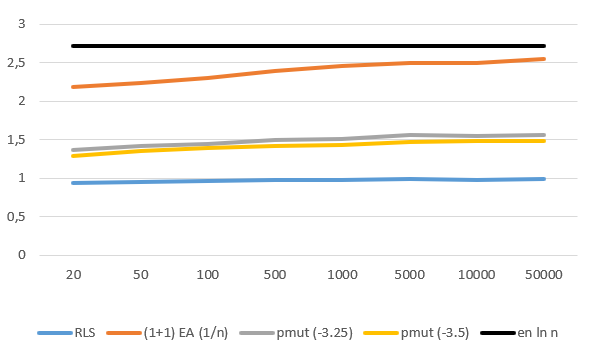
\includegraphics[width=0.7\textwidth]{figures/images/oneMaxMultipleN.png}\label{fig:onemaxNlogNBound}
\end{figure}

In a previous chapter the $\mathcal{O}(nlogn)$ bound was proven for the (1+1) EA and the RLS.
This seems to hold in practice.
\section{Carsten Witts worst case input}
C. Witt proved the RLS and the (1+1) EA find a $(4/3+\epsilon)$ approximation in expected time $\mathcal{O}(n)$ and a $(4/3)$-approximation in expected time $\mathcal{O}(n^2)$~\cite{diekert2005stacs}.
He then introduced an almost worst case input to prove the bound for the approximation ratio is at least almost tight.
The input is defined as followed for any $0<\epsilon<1/3$ and even $n$:\newline
The input contains two numbers of value $1/3 - \epsilon/4$ and n-2 elements of value $(1/3+\epsilon/2)/(n-2)$. 
The total volume is normalised to 1.
When the two large values are in the same bin, the RSHs are tricked into a local optima, where only $w_1$ and $w_2$ are in the first bin and the remaining elements in the other bin.
This results in an almost worst case.
As all researched inputs in this paper contained only integer values this input is adjusted a bit.
To prevent the small values to be below zero they are instead normalised to 1.
The two big values are scaled by the same factor of $((1/3+\epsilon/2)/(n-2))^{-1}$.
The higher the value for $\epsilon$ the more likely the input is to get stuck in the local optima.
With increasing $\epsilon$ the local optima becomes better and better.
For the small values of $\epsilon$ there were only a few cases where some algorithms did not find an optimal solution.
To make this effect more visible value was set to $\epsilon=0.3$.\newline
For $n=10,000$ this evaluates to $w_1=w_2=5344$ and $W=9998 \cdot 1 + 2 \cdot 5344 = 20686$.
The input then looks like this: $[1, 1, \dots, 1, 1, 5344, 5344]$.
The fitness of the local optimum is $f(x) = 2 \cdot 5433 = 10688$.
To leave the local optimum the algorithm therefore has to flip at least  $5433+9998-10688 = 4654$ bits as well in the same step.
The best fitness is $f(x) = 5344 + 9998/2 = 10343$, which leads to a difference of $f(localOptimum)-f(opt) = 345$ and a approximation ratio of $f(localOptimum)/f(opt)=10688/10343=1.033$.
This is not really close to the worst case of 4/3 any more but with this setting at least many algorithms are stuck in the local optimum at least once for the 1000 runs.
\subsection{RLS Comparison}


\makebox[\linewidth]{
\begin{tabular}{lp{3cm}p{6cm}p{6cm}}
\begin{tabular}[h]{cccccccc}
algo type&            \RLSN&     \RLSR&     \RLSR&     \RLSN&     \RLSR&     \RLSN&       RLS\\
algo param&             b=2&       s=3&       s=4&       b=3&       s=2&       b=4&         -\\
avg mut/change&       2.000&     1.996&     2.476&     3.000&     1.502&     4.000&     1.000\\
avg mut/step&         2.000&     2.000&     2.500&     3.000&     1.500&     4.000&     1.000\\
\hline
total avg count&     83,118&   104,748&   105,513&   112,223&   114,486&   121,927& 2,443,567\\
avg eval count&      83,118&   104,748&   105,513&   112,223&   114,486&   121,927&    45,834\\
max eval count&     778,110& 1,453,252&   898,974& 1,377,471&   915,268&   816,633&   485,275\\
min eval count&         197&       126&        45&       212&       271&       155&       128\\
\hline
fail ratio&           0.000&     0.000&     0.000&     0.000&     0.000&     0.000&     0.447\\
avg fail dif&             -&         -&         -&         -&         -&         -&         1\\
\end{tabular}
\end{tabular}
}


The RLS is by far most likely to get stuck in the local optimum.
The general tendency is the more bits the algorithm flips in expectation the more unlikely the local optimum becomes.
The only case where this does not hold is the $RLS-N_2$ being better than the $RLS-R_4$, although the $RLS-R_4$ flips more bits in expectation.
This might be caused by the higher probability for flipping only one bit for the $RLS-R_4$.
This causes the algorithm to find the local optimum faster before separating $w_1$ and $w_2$.
So the ranking of the algorithms is completely inverted compared to the OneMax input.
The $RLS-N_2$ and $RLS-N_3$ both had runs where they neither found the global nor one of the two local optima.
The algorithms were most likely tricked into the direction of the local optimum and did not manage to leave it.
But they were also not fast enough to reach the local optimum because of their low probability to flip only one bit.
\subsection{(1+1) EA Comparison}


\makebox[\linewidth]{
\begin{tabular}{lp{3cm}p{6cm}p{6cm}}
\begin{tabular}[h]{ccccccccc}
algo type&          (1+1) EA&   (1+1) EA&   (1+1) EA&   (1+1) EA&      (1+1) EA&   (1+1) EA&   (1+1) EA&   (1+1) EA\\
algo param&           3/n&     4/n&     2/n&     5/n&       -&    10/n&    50/n&   100/n\\
avg mut/change&     3.101&   3.968&   2.343&   4.859&   1.698&   9.732&  49.544&  99.494\\
avg mut/step&       2.999&   4.003&   2.002&   4.999&   1.001&   9.998&  49.998&  99.997\\
\hline
total avg count&      646&     701&     706&     857&   1,123&   1,508&   8,175&  15,485\\
avg eval count&       646&     701&     706&     857&   1,123&   1,508&   8,175&  15,485\\
max eval count&     5,346&   5,692&   3,415&   5,572&   7,001&  12,112&  52,831& 145,269\\
min eval count&        23&       4&      30&       9&      23&      14&      27&      69\\
\hline
fails&                  0&       0&       0&       0&       0&       0&       0&       0\\
fail ratio&         0.000&   0.000&   0.000&   0.000&   0.000&   0.000&   0.000&   0.000\\
avg fail dif&           -&       -&       -&       -&       -&       -&       -&       -\\
\end{tabular}
\end{tabular}
}


For the EA the result is also the inversion of the results for the OneMax equivalent.
The higher the mutation rate the faster the algorithms reach a global optimum.
This holds at least up to $p_m\le100/n$.
With mutation rate $p_m\le3/n$ the algorithm reaches the worst case at least once in 1000 runs.
If the algorithm did not manage to find an optimal solution the fitness was always the same.
So there was no run where any algorithm neither found a global nor the local optimum.
\subsection{pmut Comparison}


\makebox[\linewidth]{
\scriptsize
\begin{tabular}{lp{3cm}p{6cm}p{6cm}}
\begin{tabular}[h]{m{2.5cm}m{0,40cm}m{0,40cm}m{0,40cm}m{0,40cm}m{0,40cm}m{0,40cm}m{0,40cm}m{0,40cm}m{0,40cm}m{0,40cm}m{0,40cm}m{0,40cm}m{0,40cm}m{0,40cm}m{0,40cm}m{0,40cm}m{0,40cm}m{0,40cm}}
\multicolumn{1}{c}{algo type}&\multicolumn{2}{c}{            pmut}&\multicolumn{2}{c}{     pmut}&\multicolumn{2}{c}{     pmut}&\multicolumn{2}{c}{     pmut}&\multicolumn{2}{c}{     pmut}&\multicolumn{2}{c}{     pmut}&\multicolumn{2}{c}{     pmut}&\multicolumn{2}{c}{     pmut}&\multicolumn{2}{c}{     pmut}\\
\multicolumn{1}{c}{algo param}&\multicolumn{2}{c}{           3.25}&\multicolumn{2}{c}{     3.00}&\multicolumn{2}{c}{     2.75}&\multicolumn{2}{c}{     2.50}&\multicolumn{2}{c}{     2.25}&\multicolumn{2}{c}{     2.00}&\multicolumn{2}{c}{     1.75}&\multicolumn{2}{c}{     1.50}&\multicolumn{2}{c}{     1.25}\\
\multicolumn{1}{c}{avg mut/change}&\multicolumn{2}{c}{      1.583}&\multicolumn{2}{c}{    1.737}&\multicolumn{2}{c}{    2.002}&\multicolumn{2}{c}{    2.423}&\multicolumn{2}{c}{    3.303}&\multicolumn{2}{c}{    5.830}&\multicolumn{2}{c}{   12.519}&\multicolumn{2}{c}{   30.910}&\multicolumn{2}{c}{   73.182}\\
\multicolumn{1}{c}{avg mut/step}&\multicolumn{2}{c}{        1.729}&\multicolumn{2}{c}{    1.934}&\multicolumn{2}{c}{    2.274}&\multicolumn{2}{c}{    2.895}&\multicolumn{2}{c}{    4.360}&\multicolumn{2}{c}{    8.452}&\multicolumn{2}{c}{   22.278}&\multicolumn{2}{c}{   70.532}&\multicolumn{2}{c}{  224.421}\\
\hline
\multicolumn{1}{c}{avg eval count}&\multicolumn{2}{c}{        540}&\multicolumn{2}{c}{      569}&\multicolumn{2}{c}{      594}&\multicolumn{2}{c}{      641}&\multicolumn{2}{c}{      712}&\multicolumn{2}{c}{      808}&\multicolumn{2}{c}{      967}&\multicolumn{2}{c}{    1,285}&\multicolumn{2}{c}{    2,081}\\
\multicolumn{1}{c}{max eval count}&\multicolumn{2}{c}{      3,110}&\multicolumn{2}{c}{    2,891}&\multicolumn{2}{c}{    3,504}&\multicolumn{2}{c}{    3,896}&\multicolumn{2}{c}{    5,152}&\multicolumn{2}{c}{    4,274}&\multicolumn{2}{c}{    5,610}&\multicolumn{2}{c}{    6,190}&\multicolumn{2}{c}{   14,984}\\
\multicolumn{1}{c}{min eval count}&\multicolumn{2}{c}{         22}&\multicolumn{2}{c}{        9}&\multicolumn{2}{c}{       36}&\multicolumn{2}{c}{       25}&\multicolumn{2}{c}{       28}&\multicolumn{2}{c}{       27}&\multicolumn{2}{c}{       27}&\multicolumn{2}{c}{       13}&\multicolumn{2}{c}{       33}\\
\hline
\multicolumn{1}{c}{fail ratio}&\multicolumn{2}{c}{          0.000}&\multicolumn{2}{c}{    0.000}&\multicolumn{2}{c}{    0.000}&\multicolumn{2}{c}{    0.000}&\multicolumn{2}{c}{    0.000}&\multicolumn{2}{c}{    0.000}&\multicolumn{2}{c}{    0.000}&\multicolumn{2}{c}{    0.000}&\multicolumn{2}{c}{    0.000}\\
\hline
\multicolumn{1}{c}{p-value}&&\multicolumn{2}{c}{0.0000}&\multicolumn{2}{c}{0.0000}&\multicolumn{2}{c}{0.0000}&\multicolumn{2}{c}{0.0000}&\multicolumn{2}{c}{0.0000}&\multicolumn{2}{c}{0.0000}&\multicolumn{2}{c}{0.0000}&\multicolumn{2}{c}{0.0000}\\
&&&&&&&&&&&&&&&&&&\end{tabular}
\end{tabular}
}


For $pmut$ the result is the exact same as for the (1+1) EA.
The higher (lower absolute value) $\beta$ the better the performance as more bits are flipped in each step.
The algorithm is tricked into the local optima only for $\beta\le-2.5$.
If the algorithm is on the path to the local optimum it is always fast enough to reach it within the time limit.
\subsection{Comparison of the best variants}


\makebox[\linewidth]{
\begin{tabular}{lp{3cm}p{6cm}p{6cm}}
\begin{tabular}[h]{cccc}
algo type&            RLS&    pmut&      EA\\
algo param&             -&    3.25&       -\\
avg mut/change&     1.000&   1.287&   1.272\\
avg mut/step&       1.000&   1.729&   1.000\\
\hline
avg eval count&    91,171& 143,121& 231,082\\
max eval count&   153,143& 227,737& 446,942\\
min eval count&    65,783&  93,602& 165,818\\
\hline
fail ratio&         0.000&   0.000&   0.000\\
\end{tabular}
\end{tabular}
}


The $pmut_-1.25$ and the (1+1) EA with $p_m=100/n$ perform the best and always find an optimal solution within 600 iterations and even under 100 on the average case.
The $RLS-N_4$ performs significantly worse.
The other algorithm flip so many bits that they are almost close to random sampling.
In the experiment with different input sizes the mutation rate of $p_m=100/n$ is $\ge1$ for $n\le100$.
If the algorithm flips every bit then it won't change its solution.
In these cases the mutation rate was then set to $p_m=1/2$.

\begin{tabular}[h]{ccccccccc}
fails in 1000 runs&20&50&100&500&1000&5000&10000&50000\\\hline
RLS&984&773&411&1&0&0&0&0\\
\RLSR[2]&890&241&14&0&0&0&0&0\\
(1+1) EA (1$/n$)&711&75&5&0&0&0&0&0\\
(1+1) EA (2$/n$)&541&14&0&0&0&0&0&0\\
pmut (3.0)&566&63&4&0&0&0&0&0\\
pmut (3.25)&587&63&7&0&0&0&0&0\\
\end{tabular}


Only the RLS variant had runs where it did not reach a global optimum.
This happened in less than 0.5 \% of the inputs for $n=20$ and $n=100$.
For the other input sizes it also managed to reach a global optimum for all inputs.

\begin{tabular}[h]{ccccccccc}
avg&20&50&100&500&1000&5000&10000&50000\\\hline
RLS&32&79&153&579&950&1859&1922&1797\\
\RLSR[2]&391&2124&5005&4218&3530&2362&2160&2229\\
(1+1) EA (1$/n$)&22471&18343&12834&8342&6511&3815&3458&3371\\
(1+1) EA (2$/n$)&16360&9243&6452&4503&4020&3171&3141&3133\\
pmut (3.25)&23440&15929&9658&5644&4406&2434&2162&2172\\
pmut (3.0)&21901&14696&9186&5222&4150&2510&2208&2213\\
\end{tabular}


For the lower input sizes the RLS is slower than the remaining algorithm even it manages to find a global optimum.

\begin{tabular}[h]{ccccccccc}
total avg&20&50&100&500&1000&5000&10000&50000\\\hline
RLS&99470&93459&74385&3474&447&389&421&555\\
\RLSR[2]&96305&63088&19364&815&589&565&595&699\\
(1+1) EA (1$/n$)&89444&52886&21141&1410&869&850&875&1046\\
(1+1) EA (2$/n$)&79603&37214&14107&1302&992&942&957&1055\\
pmut (3.25)&84226&48403&18280&930&542&526&546&642\\
pmut (3.0)&82474&46286&17825&917&576&548&573&668\\
\end{tabular}



The $pmut_{-1.25}$ is the best variant closely followed by the (1+1) EA.
The RLS version is by far slower than the other to variants for the bigger input sizes.
Even for the smaller inputs it is still slower.
\section{Multiple distributions mixed}
This input does not follow a specific distribution but rather is a mix of the previous distributions.
The value is either chosen uniform random, from a binomial distribution \textasciitilde$B(10000, 0.1)$, from a geometric distribution with $p=0.001$ or a powerlaw distribution with $\beta=-2.75$.
One of the distributions is chosen uniform randomly.
This process is repeated $n$ times.
The values of this distribution then follow neither of the used distributions.

\begin{figure}[h]
      \caption{Distribution of a mixed input with \textasciitilde$U(1,999)$, \textasciitilde$B(1000.0.1)$, \textasciitilde$Geo(0.01)$, powerlaw dist with $\beta=-1.25$}
      \centering
      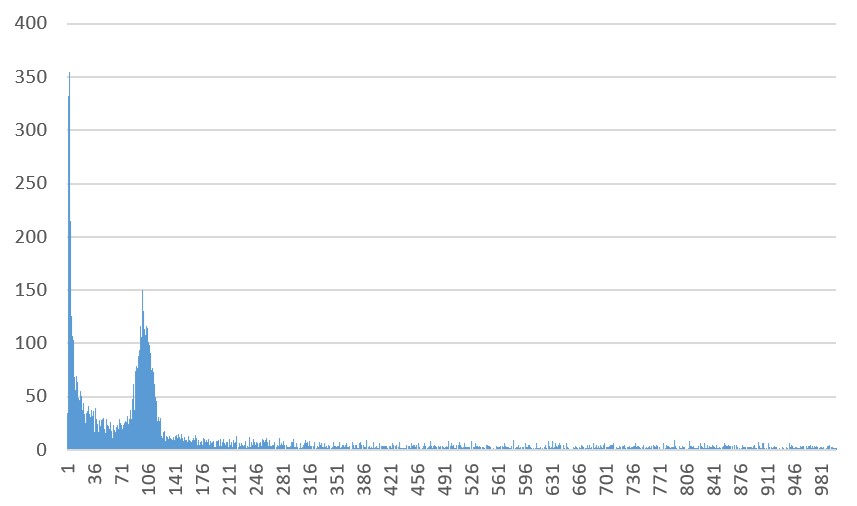
\includegraphics[width=0.7\textwidth]{figures/images/numberGenerator/mixed.png}\label{fig:mixedDistExample}
\end{figure}

The used distributions were \textasciitilde$U(1,49999)$, \textasciitilde$B(10000.0.1)$, \textasciitilde$Geo(0.001)$, powerlaw dist with $\beta=-1.25$
\subsection{RLS Comparison}


\makebox[\linewidth]{
\begin{tabular}{lp{3cm}p{6cm}p{6cm}}
\begin{tabular}[h]{cccccccc}
algo type&            \RLSN&     \RLSR&     \RLSR&     \RLSN&     \RLSR&     \RLSN&       RLS\\
algo param&             b=2&       s=3&       s=4&       b=3&       s=2&       b=4&         -\\
avg mut/change&       2.000&     1.996&     2.476&     3.000&     1.502&     4.000&     1.000\\
avg mut/step&         2.000&     2.000&     2.500&     3.000&     1.500&     4.000&     1.000\\
\hline
total avg count&     83,118&   104,748&   105,513&   112,223&   114,486&   121,927& 2,443,567\\
avg eval count&      83,118&   104,748&   105,513&   112,223&   114,486&   121,927&    45,834\\
max eval count&     778,110& 1,453,252&   898,974& 1,377,471&   915,268&   816,633&   485,275\\
min eval count&         197&       126&        45&       212&       271&       155&       128\\
\hline
fail ratio&           0.000&     0.000&     0.000&     0.000&     0.000&     0.000&     0.447\\
avg fail dif&             -&         -&         -&         -&         -&         -&         1\\
\end{tabular}
\end{tabular}
}


The results are mostly the same as for the geometric input.
The performance increases with the probability of flipping only one bit.
The main difference is the RLS being the best variant in this case as it reaches an optimal solution in every run.
The penalty of flipping only one bit is greater than for the geometric input but certainly not as drastic as for the OneMax equivalent.
By comparing the average number of iterations it seems like this input is much easier than the geometric input.
\subsection{(1+1) EA Comparison}


\makebox[\linewidth]{
\begin{tabular}{lp{3cm}p{6cm}p{6cm}}
\begin{tabular}[h]{ccccccccc}
algo type&          (1+1) EA&   (1+1) EA&   (1+1) EA&   (1+1) EA&      (1+1) EA&   (1+1) EA&   (1+1) EA&   (1+1) EA\\
algo param&           3/n&     4/n&     2/n&     5/n&       -&    10/n&    50/n&   100/n\\
avg mut/change&     3.101&   3.968&   2.343&   4.859&   1.698&   9.732&  49.544&  99.494\\
avg mut/step&       2.999&   4.003&   2.002&   4.999&   1.001&   9.998&  49.998&  99.997\\
\hline
total avg count&      646&     701&     706&     857&   1,123&   1,508&   8,175&  15,485\\
avg eval count&       646&     701&     706&     857&   1,123&   1,508&   8,175&  15,485\\
max eval count&     5,346&   5,692&   3,415&   5,572&   7,001&  12,112&  52,831& 145,269\\
min eval count&        23&       4&      30&       9&      23&      14&      27&      69\\
\hline
fails&                  0&       0&       0&       0&       0&       0&       0&       0\\
fail ratio&         0.000&   0.000&   0.000&   0.000&   0.000&   0.000&   0.000&   0.000\\
avg fail dif&           -&       -&       -&       -&       -&       -&       -&       -\\
\end{tabular}
\end{tabular}
}


For the (1+1) EA the same holds.
It performs better with decreasing mutation rate with $p_m=2/n$ being the only exception again.
The same was true for the geometric input.
The penality for the wrong parameter is also bigger for the (1+1) EA compared to the geometric input.
So the results are rather similar to the RLS.
\subsection{pmut Comparison}


\makebox[\linewidth]{
\scriptsize
\begin{tabular}{lp{3cm}p{6cm}p{6cm}}
\begin{tabular}[h]{m{2.5cm}m{0,40cm}m{0,40cm}m{0,40cm}m{0,40cm}m{0,40cm}m{0,40cm}m{0,40cm}m{0,40cm}m{0,40cm}m{0,40cm}m{0,40cm}m{0,40cm}m{0,40cm}m{0,40cm}m{0,40cm}m{0,40cm}m{0,40cm}m{0,40cm}}
\multicolumn{1}{c}{algo type}&\multicolumn{2}{c}{            pmut}&\multicolumn{2}{c}{     pmut}&\multicolumn{2}{c}{     pmut}&\multicolumn{2}{c}{     pmut}&\multicolumn{2}{c}{     pmut}&\multicolumn{2}{c}{     pmut}&\multicolumn{2}{c}{     pmut}&\multicolumn{2}{c}{     pmut}&\multicolumn{2}{c}{     pmut}\\
\multicolumn{1}{c}{algo param}&\multicolumn{2}{c}{           3.25}&\multicolumn{2}{c}{     3.00}&\multicolumn{2}{c}{     2.75}&\multicolumn{2}{c}{     2.50}&\multicolumn{2}{c}{     2.25}&\multicolumn{2}{c}{     2.00}&\multicolumn{2}{c}{     1.75}&\multicolumn{2}{c}{     1.50}&\multicolumn{2}{c}{     1.25}\\
\multicolumn{1}{c}{avg mut/change}&\multicolumn{2}{c}{      1.583}&\multicolumn{2}{c}{    1.737}&\multicolumn{2}{c}{    2.002}&\multicolumn{2}{c}{    2.423}&\multicolumn{2}{c}{    3.303}&\multicolumn{2}{c}{    5.830}&\multicolumn{2}{c}{   12.519}&\multicolumn{2}{c}{   30.910}&\multicolumn{2}{c}{   73.182}\\
\multicolumn{1}{c}{avg mut/step}&\multicolumn{2}{c}{        1.729}&\multicolumn{2}{c}{    1.934}&\multicolumn{2}{c}{    2.274}&\multicolumn{2}{c}{    2.895}&\multicolumn{2}{c}{    4.360}&\multicolumn{2}{c}{    8.452}&\multicolumn{2}{c}{   22.278}&\multicolumn{2}{c}{   70.532}&\multicolumn{2}{c}{  224.421}\\
\hline
\multicolumn{1}{c}{avg eval count}&\multicolumn{2}{c}{        540}&\multicolumn{2}{c}{      569}&\multicolumn{2}{c}{      594}&\multicolumn{2}{c}{      641}&\multicolumn{2}{c}{      712}&\multicolumn{2}{c}{      808}&\multicolumn{2}{c}{      967}&\multicolumn{2}{c}{    1,285}&\multicolumn{2}{c}{    2,081}\\
\multicolumn{1}{c}{max eval count}&\multicolumn{2}{c}{      3,110}&\multicolumn{2}{c}{    2,891}&\multicolumn{2}{c}{    3,504}&\multicolumn{2}{c}{    3,896}&\multicolumn{2}{c}{    5,152}&\multicolumn{2}{c}{    4,274}&\multicolumn{2}{c}{    5,610}&\multicolumn{2}{c}{    6,190}&\multicolumn{2}{c}{   14,984}\\
\multicolumn{1}{c}{min eval count}&\multicolumn{2}{c}{         22}&\multicolumn{2}{c}{        9}&\multicolumn{2}{c}{       36}&\multicolumn{2}{c}{       25}&\multicolumn{2}{c}{       28}&\multicolumn{2}{c}{       27}&\multicolumn{2}{c}{       27}&\multicolumn{2}{c}{       13}&\multicolumn{2}{c}{       33}\\
\hline
\multicolumn{1}{c}{fail ratio}&\multicolumn{2}{c}{          0.000}&\multicolumn{2}{c}{    0.000}&\multicolumn{2}{c}{    0.000}&\multicolumn{2}{c}{    0.000}&\multicolumn{2}{c}{    0.000}&\multicolumn{2}{c}{    0.000}&\multicolumn{2}{c}{    0.000}&\multicolumn{2}{c}{    0.000}&\multicolumn{2}{c}{    0.000}\\
\hline
\multicolumn{1}{c}{p-value}&&\multicolumn{2}{c}{0.0000}&\multicolumn{2}{c}{0.0000}&\multicolumn{2}{c}{0.0000}&\multicolumn{2}{c}{0.0000}&\multicolumn{2}{c}{0.0000}&\multicolumn{2}{c}{0.0000}&\multicolumn{2}{c}{0.0000}&\multicolumn{2}{c}{0.0000}\\
&&&&&&&&&&&&&&&&&&\end{tabular}
\end{tabular}
}


$pmut_\beta$ also performs similar to the geometric input.
Here $\beta=-3.25$ and $\beta=-3.0$ are switched instead of $\beta = -2.5$ and $-3.75$.
Apart from that the algorithm perform strictly ranked by their probability to flip only one bit per step.
Solving the mixed input is easier for the $pmut$ operator too.
All variants manage to find an optimal solution within 1000 steps on average compared to 6,200 steps for the geometric input.
The maximum number of steps is also lower by a factor of at least 10 for every value of $\beta$.
\subsection{Comparison of the best variants}


\makebox[\linewidth]{
\begin{tabular}{lp{3cm}p{6cm}p{6cm}}
\begin{tabular}[h]{cccc}
algo type&            RLS&    pmut&      EA\\
algo param&             -&    3.25&       -\\
avg mut/change&     1.000&   1.287&   1.272\\
avg mut/step&       1.000&   1.729&   1.000\\
\hline
avg eval count&    91,171& 143,121& 231,082\\
max eval count&   153,143& 227,737& 446,942\\
min eval count&    65,783&  93,602& 165,818\\
\hline
fail ratio&         0.000&   0.000&   0.000\\
\end{tabular}
\end{tabular}
}


This input seems generally easy to solve as for every base algorithm multiple variants reach an optimal solution within 1000 steps.
The standard RLS reaches an optimal solution the fastest, but the other algorithms are almost equally fast.
All algorithms finish within 501 steps on average and always in less than 2500 steps.

\begin{tabular}[h]{ccccccccc}
fails in 1000 runs&20&50&100&500&1000&5000&10000&50000\\\hline
RLS&984&773&411&1&0&0&0&0\\
\RLSR[2]&890&241&14&0&0&0&0&0\\
(1+1) EA (1$/n$)&711&75&5&0&0&0&0&0\\
(1+1) EA (2$/n$)&541&14&0&0&0&0&0&0\\
pmut (3.0)&566&63&4&0&0&0&0&0\\
pmut (3.25)&587&63&7&0&0&0&0&0\\
\end{tabular}


This input is only hard to solve for $n<100$.
Only the RLS is stuck in a local optimum for many inputs.
The other algorithms manage to escape the local optima in most cases even for $n=100$.
For $n\ge500$ every input is solved by each of the chosen algorithms except for the standard RLS failing once for $n=500$.
This is probably caused by the many small values from the powerlaw and geometric distribution.
The longer the input the more of these small values can be used to fill the gaps.

\begin{tabular}[h]{ccccccccc}
avg&20&50&100&500&1000&5000&10000&50000\\\hline
RLS&32&79&153&579&950&1859&1922&1797\\
\RLSR[2]&391&2124&5005&4218&3530&2362&2160&2229\\
(1+1) EA (1$/n$)&22471&18343&12834&8342&6511&3815&3458&3371\\
(1+1) EA (2$/n$)&16360&9243&6452&4503&4020&3171&3141&3133\\
pmut (3.25)&23440&15929&9658&5644&4406&2434&2162&2172\\
pmut (3.0)&21901&14696&9186&5222&4150&2510&2208&2213\\
\end{tabular}


The RLS variants are only able to solve the inputs if they are lucky.
The (1+1) EAs and the $pmut$ variants also find other optimal solutions but need way more steps if they do so.
The input becomes drastically easier until $n=500$ and very slowly becomes harder with rising $n$ again.

\begin{tabular}[h]{ccccccccc}
total avg&20&50&100&500&1000&5000&10000&50000\\\hline
RLS&99470&93459&74385&3474&447&389&421&555\\
\RLSR[2]&96305&63088&19364&815&589&565&595&699\\
(1+1) EA (1$/n$)&89444&52886&21141&1410&869&850&875&1046\\
(1+1) EA (2$/n$)&79603&37214&14107&1302&992&942&957&1055\\
pmut (3.25)&84226&48403&18280&930&542&526&546&642\\
pmut (3.0)&82474&46286&17825&917&576&548&573&668\\
\end{tabular}



For $n\le100$ the (1+1) EA with $p_m=2/n$ performs the best.
It is still good for the bigger values of $n$ but after $n\ge500$ $pmut_{-3.0}$ reaches an optimal solution faster.
The standard RLS is only the fastest for a small range of values but has the disadvantage of the poor performance for small inputs.
Choosing one of the other variants is a much safer choice.
\section{Multiple distributions overlapped}
This input is similar to the mixed input from the last subsection.
For this distribution the values are not chosen uniform random from one of the base distributions, but instead a value from every distribution is chosen and added together.
Hence the name overlapped distribution.
For this input the step limit was increased to $100\cdot n \ln n$.
The comparison for the step limit $10\cdot n \ln n$ is contained in only for the best algorithms.

\begin{figure}[h]
      \caption{Distribution of an overlapped input with \textasciitilde$U(1,999)$, \textasciitilde$B(1000.0.1)$, \textasciitilde$Geo(0.01)$, powerlaw dist with $\beta=-1.25$}
      \centering
      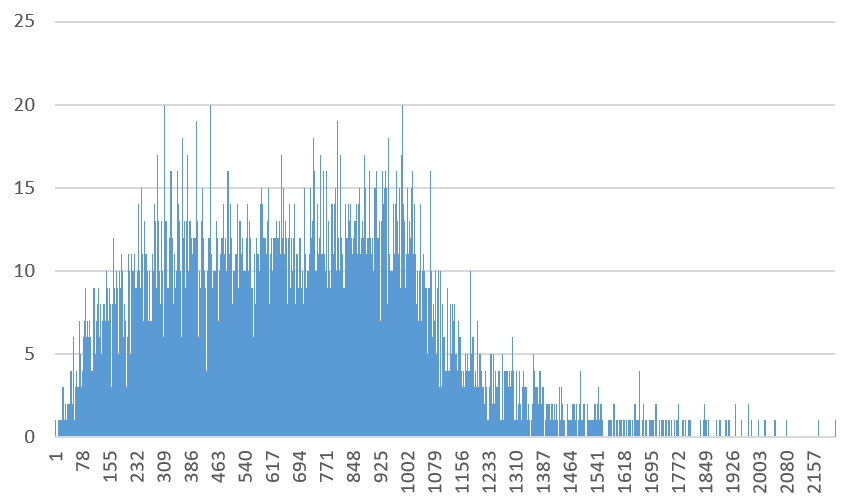
\includegraphics[width=0.7\textwidth]{figures/images/numberGenerator/overlapped.png}\label{fig:overlappedDistExample}
\end{figure}

The used distributions were \textasciitilde$U(1,49999)$, \textasciitilde$B(10000.0.1)$, \textasciitilde$Geo(0.001)$, powerlaw dist with $\beta=-1.25$
\subsection{RLS Comparison}


\makebox[\linewidth]{
\begin{tabular}{lp{3cm}p{6cm}p{6cm}}
\begin{tabular}[h]{cccccccc}
algo type&            \RLSN&     \RLSR&     \RLSR&     \RLSN&     \RLSR&     \RLSN&       RLS\\
algo param&             b=2&       s=3&       s=4&       b=3&       s=2&       b=4&         -\\
avg mut/change&       2.000&     1.996&     2.476&     3.000&     1.502&     4.000&     1.000\\
avg mut/step&         2.000&     2.000&     2.500&     3.000&     1.500&     4.000&     1.000\\
\hline
total avg count&     83,118&   104,748&   105,513&   112,223&   114,486&   121,927& 2,443,567\\
avg eval count&      83,118&   104,748&   105,513&   112,223&   114,486&   121,927&    45,834\\
max eval count&     778,110& 1,453,252&   898,974& 1,377,471&   915,268&   816,633&   485,275\\
min eval count&         197&       126&        45&       212&       271&       155&       128\\
\hline
fail ratio&           0.000&     0.000&     0.000&     0.000&     0.000&     0.000&     0.447\\
avg fail dif&             -&         -&         -&         -&         -&         -&         1\\
\end{tabular}
\end{tabular}
}


The results for this distribution are rather similar to the results of the binomial distribution.
The ranking of the algorithms is completely the same.
Only the RLS almost fails to find an optimal solution for almost every input.
For the binomial distribution the $RLS-N_3$ also failed around 25\% or the inputs but here it does not.
Another big difference is the number of steps needed to find a global optimum.
For the binomial input all algorithms except the RLS were really fast and only needed below 1000 iterations on average.
All algorithm need around 500 times the number of steps on average as compared to the binomial inputs.
\subsection{(1+1) EA Comparison}


\makebox[\linewidth]{
\begin{tabular}{lp{3cm}p{6cm}p{6cm}}
\begin{tabular}[h]{ccccccccc}
algo type&          (1+1) EA&   (1+1) EA&   (1+1) EA&   (1+1) EA&      (1+1) EA&   (1+1) EA&   (1+1) EA&   (1+1) EA\\
algo param&           3/n&     4/n&     2/n&     5/n&       -&    10/n&    50/n&   100/n\\
avg mut/change&     3.101&   3.968&   2.343&   4.859&   1.698&   9.732&  49.544&  99.494\\
avg mut/step&       2.999&   4.003&   2.002&   4.999&   1.001&   9.998&  49.998&  99.997\\
\hline
total avg count&      646&     701&     706&     857&   1,123&   1,508&   8,175&  15,485\\
avg eval count&       646&     701&     706&     857&   1,123&   1,508&   8,175&  15,485\\
max eval count&     5,346&   5,692&   3,415&   5,572&   7,001&  12,112&  52,831& 145,269\\
min eval count&        23&       4&      30&       9&      23&      14&      27&      69\\
\hline
fails&                  0&       0&       0&       0&       0&       0&       0&       0\\
fail ratio&         0.000&   0.000&   0.000&   0.000&   0.000&   0.000&   0.000&   0.000\\
avg fail dif&           -&       -&       -&       -&       -&       -&       -&       -\\
\end{tabular}
\end{tabular}
}


The results for the (1+1) EA are similar but not the same.
Algorithms that had a good runtime on binomial inputs also have a good runtime in the overlapped runs, but the ranking is not the same.
For this input every the first and second place switched, the same for 3rd and 4th and also for 5th and 6th place.
This may be only caused by chance and the performance within a pair being really close but might also be caused by something else.
The (1+1) EA variants also needed about 200 times as long as for the binomial inputs.
All runs had at least 2 runs where they did not find an optimal solution.
These runs all had a remaining difference of one to the optimal value.
More time would probably be enough to reach an optimal solution in most cases.
\subsection{pmut Comparison}


\makebox[\linewidth]{
\scriptsize
\begin{tabular}{lp{3cm}p{6cm}p{6cm}}
\begin{tabular}[h]{m{2.5cm}m{0,40cm}m{0,40cm}m{0,40cm}m{0,40cm}m{0,40cm}m{0,40cm}m{0,40cm}m{0,40cm}m{0,40cm}m{0,40cm}m{0,40cm}m{0,40cm}m{0,40cm}m{0,40cm}m{0,40cm}m{0,40cm}m{0,40cm}m{0,40cm}}
\multicolumn{1}{c}{algo type}&\multicolumn{2}{c}{            pmut}&\multicolumn{2}{c}{     pmut}&\multicolumn{2}{c}{     pmut}&\multicolumn{2}{c}{     pmut}&\multicolumn{2}{c}{     pmut}&\multicolumn{2}{c}{     pmut}&\multicolumn{2}{c}{     pmut}&\multicolumn{2}{c}{     pmut}&\multicolumn{2}{c}{     pmut}\\
\multicolumn{1}{c}{algo param}&\multicolumn{2}{c}{           3.25}&\multicolumn{2}{c}{     3.00}&\multicolumn{2}{c}{     2.75}&\multicolumn{2}{c}{     2.50}&\multicolumn{2}{c}{     2.25}&\multicolumn{2}{c}{     2.00}&\multicolumn{2}{c}{     1.75}&\multicolumn{2}{c}{     1.50}&\multicolumn{2}{c}{     1.25}\\
\multicolumn{1}{c}{avg mut/change}&\multicolumn{2}{c}{      1.583}&\multicolumn{2}{c}{    1.737}&\multicolumn{2}{c}{    2.002}&\multicolumn{2}{c}{    2.423}&\multicolumn{2}{c}{    3.303}&\multicolumn{2}{c}{    5.830}&\multicolumn{2}{c}{   12.519}&\multicolumn{2}{c}{   30.910}&\multicolumn{2}{c}{   73.182}\\
\multicolumn{1}{c}{avg mut/step}&\multicolumn{2}{c}{        1.729}&\multicolumn{2}{c}{    1.934}&\multicolumn{2}{c}{    2.274}&\multicolumn{2}{c}{    2.895}&\multicolumn{2}{c}{    4.360}&\multicolumn{2}{c}{    8.452}&\multicolumn{2}{c}{   22.278}&\multicolumn{2}{c}{   70.532}&\multicolumn{2}{c}{  224.421}\\
\hline
\multicolumn{1}{c}{avg eval count}&\multicolumn{2}{c}{        540}&\multicolumn{2}{c}{      569}&\multicolumn{2}{c}{      594}&\multicolumn{2}{c}{      641}&\multicolumn{2}{c}{      712}&\multicolumn{2}{c}{      808}&\multicolumn{2}{c}{      967}&\multicolumn{2}{c}{    1,285}&\multicolumn{2}{c}{    2,081}\\
\multicolumn{1}{c}{max eval count}&\multicolumn{2}{c}{      3,110}&\multicolumn{2}{c}{    2,891}&\multicolumn{2}{c}{    3,504}&\multicolumn{2}{c}{    3,896}&\multicolumn{2}{c}{    5,152}&\multicolumn{2}{c}{    4,274}&\multicolumn{2}{c}{    5,610}&\multicolumn{2}{c}{    6,190}&\multicolumn{2}{c}{   14,984}\\
\multicolumn{1}{c}{min eval count}&\multicolumn{2}{c}{         22}&\multicolumn{2}{c}{        9}&\multicolumn{2}{c}{       36}&\multicolumn{2}{c}{       25}&\multicolumn{2}{c}{       28}&\multicolumn{2}{c}{       27}&\multicolumn{2}{c}{       27}&\multicolumn{2}{c}{       13}&\multicolumn{2}{c}{       33}\\
\hline
\multicolumn{1}{c}{fail ratio}&\multicolumn{2}{c}{          0.000}&\multicolumn{2}{c}{    0.000}&\multicolumn{2}{c}{    0.000}&\multicolumn{2}{c}{    0.000}&\multicolumn{2}{c}{    0.000}&\multicolumn{2}{c}{    0.000}&\multicolumn{2}{c}{    0.000}&\multicolumn{2}{c}{    0.000}&\multicolumn{2}{c}{    0.000}\\
\hline
\multicolumn{1}{c}{p-value}&&\multicolumn{2}{c}{0.0000}&\multicolumn{2}{c}{0.0000}&\multicolumn{2}{c}{0.0000}&\multicolumn{2}{c}{0.0000}&\multicolumn{2}{c}{0.0000}&\multicolumn{2}{c}{0.0000}&\multicolumn{2}{c}{0.0000}&\multicolumn{2}{c}{0.0000}\\
&&&&&&&&&&&&&&&&&&\end{tabular}
\end{tabular}
}


For $pmut$ the results are mostly the same as for the (1+1) EA.
The performance is about 250 times worse than for the binomial inputs, but the ranking is still pretty close.
Here the optimal parameter is around $\beta=-1.75$ instead of $\beta=-2.25$.
For $pmut$ the step limit was too small as well, but the difference to the optimal solution was only one on average.
\subsection{Comparison of the best variants}


\makebox[\linewidth]{
\begin{tabular}{lp{3cm}p{6cm}p{6cm}}
\begin{tabular}[h]{cccc}
algo type&            RLS&    pmut&      EA\\
algo param&             -&    3.25&       -\\
avg mut/change&     1.000&   1.287&   1.272\\
avg mut/step&       1.000&   1.729&   1.000\\
\hline
avg eval count&    91,171& 143,121& 231,082\\
max eval count&   153,143& 227,737& 446,942\\
min eval count&    65,783&  93,602& 165,818\\
\hline
fail ratio&         0.000&   0.000&   0.000\\
\end{tabular}
\end{tabular}
}


The results here are the same as for the binomial input. The $RLS-N_2$ performs better than the (1+1) EA and $pmut_\beta$ mutation for all values of $c/n$ and $\beta$ by a factor of 1.5 with a step limit of $10 \cdot n \ln(n)$. For the lower values of $n$ this does not hold to that extreme.

\begin{tabular}[h]{ccccccccc}
fails in 1000 runs&20&50&100&500&1000&5000&10000&50000\\\hline
RLS&984&773&411&1&0&0&0&0\\
\RLSR[2]&890&241&14&0&0&0&0&0\\
(1+1) EA (1$/n$)&711&75&5&0&0&0&0&0\\
(1+1) EA (2$/n$)&541&14&0&0&0&0&0&0\\
pmut (3.0)&566&63&4&0&0&0&0&0\\
pmut (3.25)&587&63&7&0&0&0&0&0\\
\end{tabular}


Here almost no algorithm manages to find an optimal solution in most cases as all algorithms fail for more than 80 \% of the inputs.
The RLS variants perform the worst again for the small input sizes.
Only for $n\ge500$ the $RLS-N_{2}$ is a good option due to the hug performance increase between $n=100$ and $n=500$.
Overlapped inputs stay hard to solve relatively long as only for $n\ge50,000$ all best variants of each algorithm find an optimal solution for every input.

\begin{tabular}[h]{ccccccccc}
avg&20&50&100&500&1000&5000&10000&50000\\\hline
RLS&32&79&153&579&950&1859&1922&1797\\
\RLSR[2]&391&2124&5005&4218&3530&2362&2160&2229\\
(1+1) EA (1$/n$)&22471&18343&12834&8342&6511&3815&3458&3371\\
(1+1) EA (2$/n$)&16360&9243&6452&4503&4020&3171&3141&3133\\
pmut (3.25)&23440&15929&9658&5644&4406&2434&2162&2172\\
pmut (3.0)&21901&14696&9186&5222&4150&2510&2208&2213\\
\end{tabular}


For $n\le1000$ the performance seems almost constant, but this is caused by the constant step limit of 100,000.
After $n=1000$ the value of $10 \cdot n \ln(n)$ was bigger than 100,000.

\begin{tabular}[h]{ccccccccc}
total avg&20&50&100&500&1000&5000&10000&50000\\\hline
RLS&99470&93459&74385&3474&447&389&421&555\\
\RLSR[2]&96305&63088&19364&815&589&565&595&699\\
(1+1) EA (1$/n$)&89444&52886&21141&1410&869&850&875&1046\\
(1+1) EA (2$/n$)&79603&37214&14107&1302&992&942&957&1055\\
pmut (3.25)&84226&48403&18280&930&542&526&546&642\\
pmut (3.0)&82474&46286&17825&917&576&548&573&668\\
\end{tabular}



No algorithm is very successful for the small values of N.
Choosing the (1+1) EA for $n<500$ should result in the best runtime in most of the cases.
Only the $RLS-N_4$ is faster for $50\le n \le 100$.
For bigger input sizes the $RLS-N_2$ is clearly the best option.
\section{Multiple distributions mixed \& overlapped}
This distribution is again similar to the mixed distribution.
With probability 1/2 the value is chosen from the overlapped distribution and with remaining probability 1/2 the value is chosen from the mixed distribution.

\begin{figure}[h]
      \caption{Distribution of a mixed and overlapped input with \textasciitilde$U(1,999)$, \textasciitilde$B(1000.0.1)$, \textasciitilde$Geo(0.01)$, powerlaw dist with $\beta=-1.25$}
      \centering
      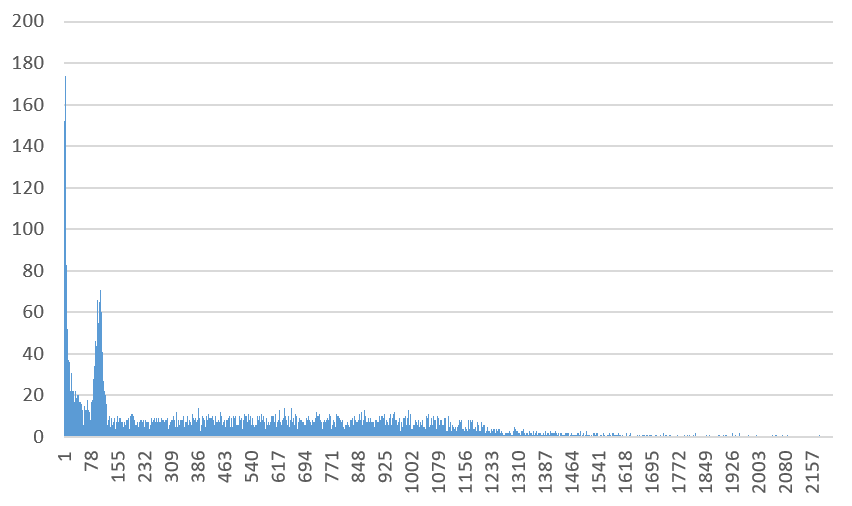
\includegraphics[width=0.7\textwidth]{figures/images/numberGenerator/mixedAndOverlapped.png}\label{fig:mixAndOverlDistExample}
\end{figure}

The used distributions were \textasciitilde$U(1,49999)$, \textasciitilde$B(10000.0.1)$, \textasciitilde$Geo(0.001)$, powerlaw dist with $\beta=-1.25$.
By looking at Figure~\ref{fig:mixAndOverlDistExample} it looks like the mixed and overlapped distribution is closer to the mixed distribution than to the overlapped distribution.
The results should also be closer to the mixed distribution.
\subsection{RLS Comparison}


\makebox[\linewidth]{
\begin{tabular}{lp{3cm}p{6cm}p{6cm}}
\begin{tabular}[h]{cccccccc}
algo type&            \RLSN&     \RLSR&     \RLSR&     \RLSN&     \RLSR&     \RLSN&       RLS\\
algo param&             b=2&       s=3&       s=4&       b=3&       s=2&       b=4&         -\\
avg mut/change&       2.000&     1.996&     2.476&     3.000&     1.502&     4.000&     1.000\\
avg mut/step&         2.000&     2.000&     2.500&     3.000&     1.500&     4.000&     1.000\\
\hline
total avg count&     83,118&   104,748&   105,513&   112,223&   114,486&   121,927& 2,443,567\\
avg eval count&      83,118&   104,748&   105,513&   112,223&   114,486&   121,927&    45,834\\
max eval count&     778,110& 1,453,252&   898,974& 1,377,471&   915,268&   816,633&   485,275\\
min eval count&         197&       126&        45&       212&       271&       155&       128\\
\hline
fail ratio&           0.000&     0.000&     0.000&     0.000&     0.000&     0.000&     0.447\\
avg fail dif&             -&         -&         -&         -&         -&         -&         1\\
\end{tabular}
\end{tabular}
}


As expected the results are similar to the mixed input.
There is a clear preference of algorithms with higher probability to flip only one bit per step.
Mixed and geometric distributions did not lead to very bad performance for the $RLS-N_4$.
The mixed and overlapped input punishes the worse mutation operators more than the other two inputs.
In that sense this type of input is closer to the OneMax equivalent, but still way less extreme.
Here still every variant reaches an optimal solution in every case.
\subsection{(1+1) EA Comparison}


\makebox[\linewidth]{
\begin{tabular}{lp{3cm}p{6cm}p{6cm}}
\begin{tabular}[h]{ccccccccc}
algo type&          (1+1) EA&   (1+1) EA&   (1+1) EA&   (1+1) EA&      (1+1) EA&   (1+1) EA&   (1+1) EA&   (1+1) EA\\
algo param&           3/n&     4/n&     2/n&     5/n&       -&    10/n&    50/n&   100/n\\
avg mut/change&     3.101&   3.968&   2.343&   4.859&   1.698&   9.732&  49.544&  99.494\\
avg mut/step&       2.999&   4.003&   2.002&   4.999&   1.001&   9.998&  49.998&  99.997\\
\hline
total avg count&      646&     701&     706&     857&   1,123&   1,508&   8,175&  15,485\\
avg eval count&       646&     701&     706&     857&   1,123&   1,508&   8,175&  15,485\\
max eval count&     5,346&   5,692&   3,415&   5,572&   7,001&  12,112&  52,831& 145,269\\
min eval count&        23&       4&      30&       9&      23&      14&      27&      69\\
\hline
fails&                  0&       0&       0&       0&       0&       0&       0&       0\\
fail ratio&         0.000&   0.000&   0.000&   0.000&   0.000&   0.000&   0.000&   0.000\\
avg fail dif&           -&       -&       -&       -&       -&       -&       -&       -\\
\end{tabular}
\end{tabular}
}


The results here are pretty similar to the results of the RLS.
The lower mutation rates perform better and higher mutation rates start to perform worse in comparison to the mixed input.
\subsection{pmut Comparison}


\makebox[\linewidth]{
\scriptsize
\begin{tabular}{lp{3cm}p{6cm}p{6cm}}
\begin{tabular}[h]{m{2.5cm}m{0,40cm}m{0,40cm}m{0,40cm}m{0,40cm}m{0,40cm}m{0,40cm}m{0,40cm}m{0,40cm}m{0,40cm}m{0,40cm}m{0,40cm}m{0,40cm}m{0,40cm}m{0,40cm}m{0,40cm}m{0,40cm}m{0,40cm}m{0,40cm}}
\multicolumn{1}{c}{algo type}&\multicolumn{2}{c}{            pmut}&\multicolumn{2}{c}{     pmut}&\multicolumn{2}{c}{     pmut}&\multicolumn{2}{c}{     pmut}&\multicolumn{2}{c}{     pmut}&\multicolumn{2}{c}{     pmut}&\multicolumn{2}{c}{     pmut}&\multicolumn{2}{c}{     pmut}&\multicolumn{2}{c}{     pmut}\\
\multicolumn{1}{c}{algo param}&\multicolumn{2}{c}{           3.25}&\multicolumn{2}{c}{     3.00}&\multicolumn{2}{c}{     2.75}&\multicolumn{2}{c}{     2.50}&\multicolumn{2}{c}{     2.25}&\multicolumn{2}{c}{     2.00}&\multicolumn{2}{c}{     1.75}&\multicolumn{2}{c}{     1.50}&\multicolumn{2}{c}{     1.25}\\
\multicolumn{1}{c}{avg mut/change}&\multicolumn{2}{c}{      1.583}&\multicolumn{2}{c}{    1.737}&\multicolumn{2}{c}{    2.002}&\multicolumn{2}{c}{    2.423}&\multicolumn{2}{c}{    3.303}&\multicolumn{2}{c}{    5.830}&\multicolumn{2}{c}{   12.519}&\multicolumn{2}{c}{   30.910}&\multicolumn{2}{c}{   73.182}\\
\multicolumn{1}{c}{avg mut/step}&\multicolumn{2}{c}{        1.729}&\multicolumn{2}{c}{    1.934}&\multicolumn{2}{c}{    2.274}&\multicolumn{2}{c}{    2.895}&\multicolumn{2}{c}{    4.360}&\multicolumn{2}{c}{    8.452}&\multicolumn{2}{c}{   22.278}&\multicolumn{2}{c}{   70.532}&\multicolumn{2}{c}{  224.421}\\
\hline
\multicolumn{1}{c}{avg eval count}&\multicolumn{2}{c}{        540}&\multicolumn{2}{c}{      569}&\multicolumn{2}{c}{      594}&\multicolumn{2}{c}{      641}&\multicolumn{2}{c}{      712}&\multicolumn{2}{c}{      808}&\multicolumn{2}{c}{      967}&\multicolumn{2}{c}{    1,285}&\multicolumn{2}{c}{    2,081}\\
\multicolumn{1}{c}{max eval count}&\multicolumn{2}{c}{      3,110}&\multicolumn{2}{c}{    2,891}&\multicolumn{2}{c}{    3,504}&\multicolumn{2}{c}{    3,896}&\multicolumn{2}{c}{    5,152}&\multicolumn{2}{c}{    4,274}&\multicolumn{2}{c}{    5,610}&\multicolumn{2}{c}{    6,190}&\multicolumn{2}{c}{   14,984}\\
\multicolumn{1}{c}{min eval count}&\multicolumn{2}{c}{         22}&\multicolumn{2}{c}{        9}&\multicolumn{2}{c}{       36}&\multicolumn{2}{c}{       25}&\multicolumn{2}{c}{       28}&\multicolumn{2}{c}{       27}&\multicolumn{2}{c}{       27}&\multicolumn{2}{c}{       13}&\multicolumn{2}{c}{       33}\\
\hline
\multicolumn{1}{c}{fail ratio}&\multicolumn{2}{c}{          0.000}&\multicolumn{2}{c}{    0.000}&\multicolumn{2}{c}{    0.000}&\multicolumn{2}{c}{    0.000}&\multicolumn{2}{c}{    0.000}&\multicolumn{2}{c}{    0.000}&\multicolumn{2}{c}{    0.000}&\multicolumn{2}{c}{    0.000}&\multicolumn{2}{c}{    0.000}\\
\hline
\multicolumn{1}{c}{p-value}&&\multicolumn{2}{c}{0.0000}&\multicolumn{2}{c}{0.0000}&\multicolumn{2}{c}{0.0000}&\multicolumn{2}{c}{0.0000}&\multicolumn{2}{c}{0.0000}&\multicolumn{2}{c}{0.0000}&\multicolumn{2}{c}{0.0000}&\multicolumn{2}{c}{0.0000}\\
&&&&&&&&&&&&&&&&&&\end{tabular}
\end{tabular}
}


Here the same holds.
The higher mutation rates are less impacted than the higher rates for the RLS and the (1+1) EA.
\subsection{Comparison of the best variants}


\makebox[\linewidth]{
\begin{tabular}{lp{3cm}p{6cm}p{6cm}}
\begin{tabular}[h]{cccc}
algo type&            RLS&    pmut&      EA\\
algo param&             -&    3.25&       -\\
avg mut/change&     1.000&   1.287&   1.272\\
avg mut/step&       1.000&   1.729&   1.000\\
\hline
avg eval count&    91,171& 143,121& 231,082\\
max eval count&   153,143& 227,737& 446,942\\
min eval count&    65,783&  93,602& 165,818\\
\hline
fail ratio&         0.000&   0.000&   0.000\\
\end{tabular}
\end{tabular}
}


The ranking of the algorithm is the same as for the other inputs with a similar preference of low mutation rates.
The RLS has the best performance closely follow by $pmut_{-3.25}$ and lastly be the standard (1+1) EA.

\begin{tabular}[h]{ccccccccc}
fails in 1000 runs&20&50&100&500&1000&5000&10000&50000\\\hline
RLS&984&773&411&1&0&0&0&0\\
\RLSR[2]&890&241&14&0&0&0&0&0\\
(1+1) EA (1$/n$)&711&75&5&0&0&0&0&0\\
(1+1) EA (2$/n$)&541&14&0&0&0&0&0&0\\
pmut (3.0)&566&63&4&0&0&0&0&0\\
pmut (3.25)&587&63&7&0&0&0&0&0\\
\end{tabular}


No unexpected results for the different input sizes.
The RLS variants perform the worst for $n\le 100$.
The input is also rather hard to solve for $n\le50$ but not as hard as the overlapped distributed input for example.

\begin{tabular}[h]{ccccccccc}
avg&20&50&100&500&1000&5000&10000&50000\\\hline
RLS&32&79&153&579&950&1859&1922&1797\\
\RLSR[2]&391&2124&5005&4218&3530&2362&2160&2229\\
(1+1) EA (1$/n$)&22471&18343&12834&8342&6511&3815&3458&3371\\
(1+1) EA (2$/n$)&16360&9243&6452&4503&4020&3171&3141&3133\\
pmut (3.25)&23440&15929&9658&5644&4406&2434&2162&2172\\
pmut (3.0)&21901&14696&9186&5222&4150&2510&2208&2213\\
\end{tabular}


The input gets easier to solve up until $n=5000$ and from then on gets harder again with increasing input size.
The increase for larger input sizes is much smaller than the decrease for the small values.

\begin{tabular}[h]{ccccccccc}
total avg&20&50&100&500&1000&5000&10000&50000\\\hline
RLS&99470&93459&74385&3474&447&389&421&555\\
\RLSR[2]&96305&63088&19364&815&589&565&595&699\\
(1+1) EA (1$/n$)&89444&52886&21141&1410&869&850&875&1046\\
(1+1) EA (2$/n$)&79603&37214&14107&1302&992&942&957&1055\\
pmut (3.25)&84226&48403&18280&930&542&526&546&642\\
pmut (3.0)&82474&46286&17825&917&576&548&573&668\\
\end{tabular}



Mixed and overlapped inputs are best solved by the (1+1) EA with $p_m=2/n$ for $n\le100$ and also relatively good for $n=500$.
After $n\ge1000$ the standard RLS becomes the best option and it seems like it stays that way for the remaining input sizes.
